\documentclass[reprint, nobibnotes, amssymb, amsmath, amsfonts, physics, mathtools, mathrsfs, floatfix]{revtex4-1}
\usepackage{graphicx}
\usepackage[english]{babel}


\newcommand{\redchi}{$\tilde{\chi}^2\,$}

\begin{document}

  \title{Relativistic Dispersion of Free Electrons}

  \author{Aman LaChapelle}
  \affiliation{The University of Chicago}


  \begin{abstract}
    We use a high-purity Germanium detector to measure with high precision the energies of incoming photons in the radiation spectrum.  We measure the kinetic energy of electrons from which these incoming photons scatter to determine the relativistic limit of the electronic dispersion relation in Ge crystal.  We determine that the well known special relativistic energy-momentum relation holds with remarkable accuracy, the model returning values of $\frac{m}{m_e} = 0.9696 \pm 0.0007$ and $2B = 1.019 \pm 0.001$.  B is the linear slope parameter that we use to characterize the relativistic mass, $\frac{p^2c^2}{2T} = BT + C$.  We finally examine the velocity and plot the dispersion relation of the electron moving with nontrivial fractions of $c$ in a Ge crystal.  We measure a rest mass for the electron of $0.5003\pm0.0001$ MeV.
  \end{abstract}

  \maketitle
  \tableofcontents

  \section{Introduction and Theory}
    The goal we seek here is to verify the relativistic dispersion relation.  In general, we can reasonably take the dispersion relation to be the nearly free electron model, especially in the case of relativistic electrons.  When the kinetic energy of an electron is such that its velocity exceeds trivial fractions of $c$, the free electron approximation works exceedingly well as a basic picture of the band structure.  Thus, we are measuring the linear part of the electron's dispersion relation in order to determine the coefficients.  In essence, as the electron moves faster, we see the band flatten into a line from the parabolic structure that we expect from a typical electron.  In performing the detection, we make use of a high-purity Germanium crystal which gives us excellent energy resolution.

    \hspace{.25cm}

    The electron energy after a high-energy scattering is given by the Compton Edge - this feature represents the energy of a photon that has undergone scattering with an electron with an angle of $\pi$ exactly once.  We can determine the momentum of the electron given this information because the energy deposited by the photon will be exactly the excess energy given to the electron.  Furthermore, we know that since Germanium has, to a good approximation, a tight-binding band structure, the electron will be both (mostly) stationary - in that it is tightly bound to its lattice site, and that once we excite it we will only see electrons interacting with the excited electron that are directly in its path.~\cite{germanium_structure}  This means that the signal we see is proportional to a number of electrons that is quite specific to the energy of the initial electron's collision.

    \begin{figure}[h]
      \centering
      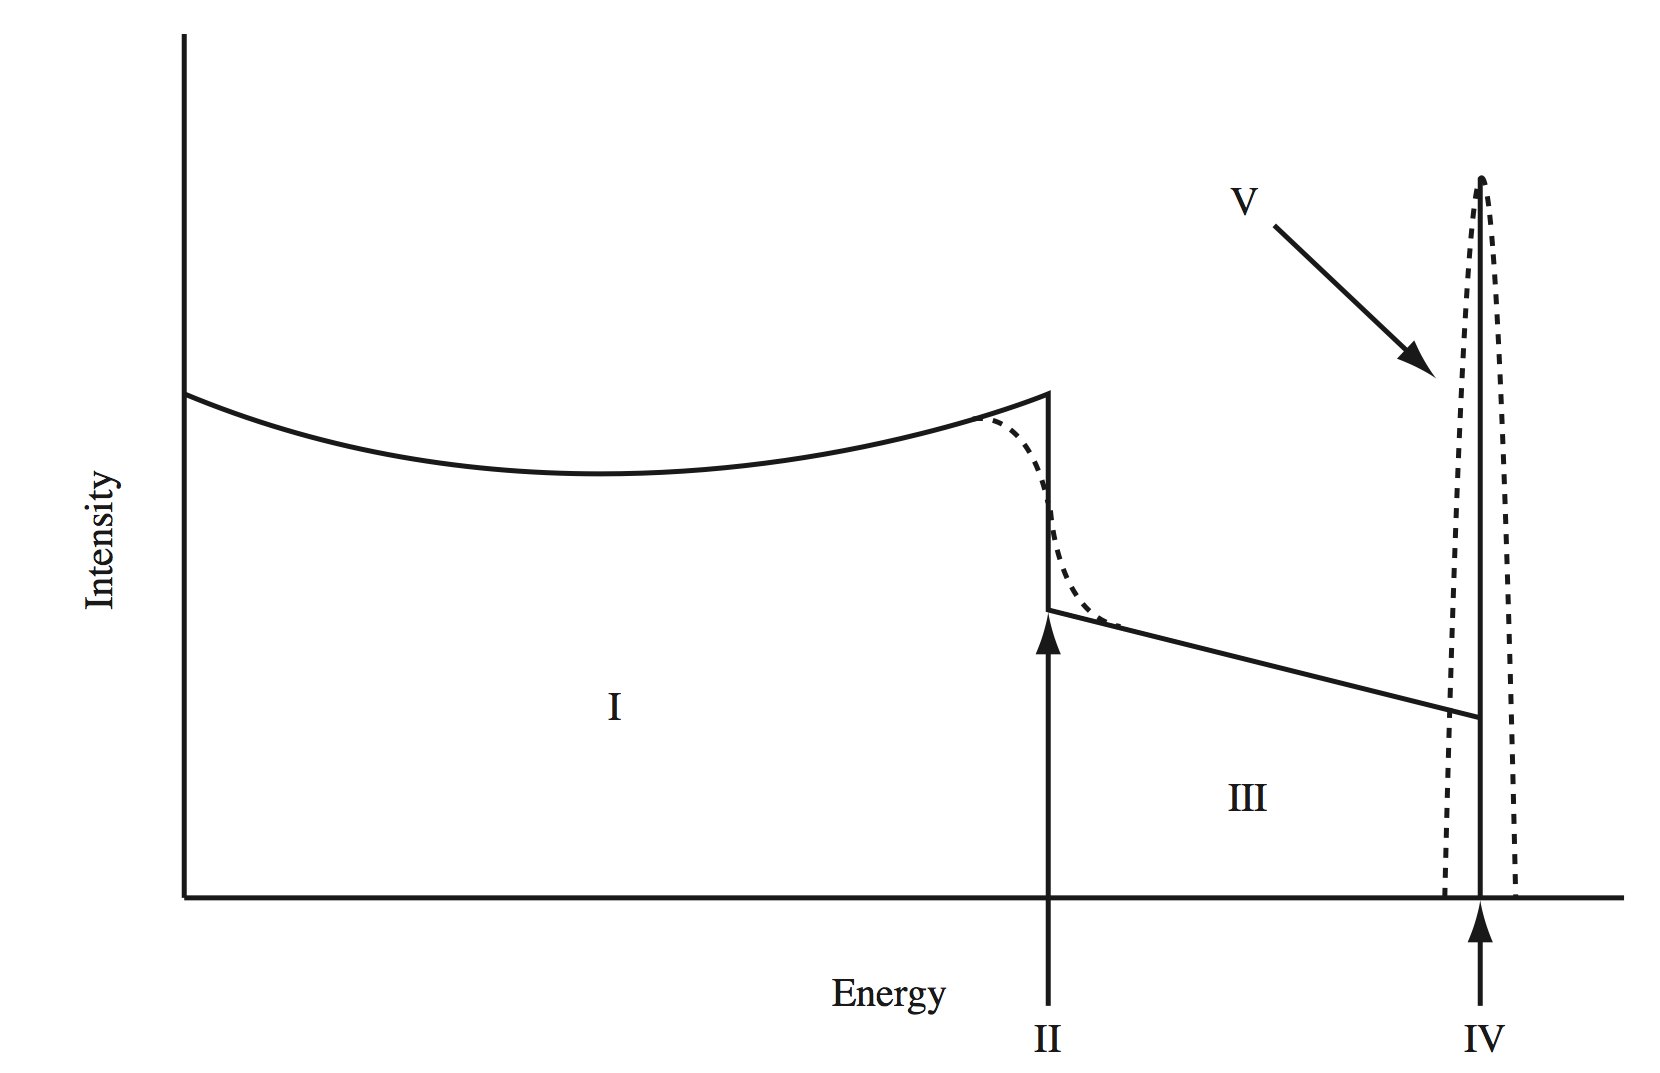
\includegraphics[width=\linewidth]{energy_spectrum.png}
      \caption{We are mainly concerned with features II and IV - these will tell us the electron energy after the compton scattering and the direct incoming photon energy (by measuring full captures - photons that scatter enough to lose all their energy), respectively.~\cite{lab_manual} \label{fig:labeled_spectrum}}
    \end{figure}

    In order to find the electrons' momentum from a detector that is very sensitive to energy, we will use conservation of energy in order to show that we can extract the electron's kinetic energy from the photon energies after scattering once and the photon direct incoming energy.  We start by realizing that the energy at the full peak is equal to the energy of the photon after scattering plus the kinetic energy imparted to the electron, giving us the following relations.

    \begin{gather}
      E_\gamma = E_\gamma ' + T \\
      \text{Turning this into momentum using $E = pc$}\nonumber\\
      \frac{E_\gamma}{c} = p - \frac{E_\gamma '}{c} \\
      \text{Therefore we have for the electron momentum}\nonumber\\
      pc = 2E_\gamma - T
    \end{gather}

    Now that we have the electron's momentum after a scattering event, we will be able to determine its dispersion relation using quantities that we can measure, namely, $E_\gamma$ and $T$.

    \hspace{.25cm}

    In order to 'discover' the special relativistic dispersion relation, we will plot the classical non-relativistic mass and see that it changes as a function of energy.  Namely, we take the following to be true:

    \begin{gather}
      T = \frac{p^2}{2m_e} \\
      \frac{p^2c^2}{2T} = m_ec^2 \label{eq:rel_mass}
    \end{gather}

    or so we would hope.  We will see that this is not, in fact, constant as we would expect and thus we will find that the actual relation is something more like the following:

    \begin{gather}
      \frac{p^2c^2}{2T} = BT + C \label{eq:fitfn} \\
      B = 1/2 \\
      C = m_ec^2 \\
      \text{which would imply the following:}\nonumber \\
      p^2c^2 = 2m_ec^2 T + T^2 \label{eq:rel_dispersion}
    \end{gather}

    which is the well-known relativistic dispersion relation.  We can see that in the limit where $T << 2m_ec^2$ we recover the classical relation where $\frac{p^2}{2T}$ reduces to the electron rest mass.  As a further bonus, when we take the same limit we can also see that the classical quadratic dispersion is recovered as well - $T = \frac{p^2}{2m}$.

    \hspace{.25cm}

    Now that we have established the relativistic form of the dispersion relation, we will explore its consequences.  The first thing that we can do is to calculate and compare the electron's rest mass as follows:
    \begin{equation}
      m_ec^2 = \frac{2E_\gamma(E_\gamma - T)}{T} \label{eq:rest_mass}
    \end{equation}

    Another quantity of interest is the velocity of the electron.  We can show that the following holds ($c = 1$):
    \begin{equation}
      \beta = \frac{T(2E_\gamma - T)}{T^2 - 2E_\gamma T + 2E_\gamma^2} \label{eq:velocity}
    \end{equation}
    and uncertainty given by:
    \begin{equation}
      \Delta \beta = \frac{4E_\gamma(E_\gamma - T)\sqrt{(E_\gamma \Delta T)^2 + (T \Delta E_\gamma)^2}}{(T^2 - 2E_\gamma T + 2E_\gamma^2)^2}. \label{eq:dvelocity}
    \end{equation}

    We will also need the relativistic forms of the momentum and kinetic energy, given respectively by:
    \begin{equation}
      pc = \frac{m_ec^2\beta}{\sqrt{1-\beta^2}} \label{eq:momentum}
    \end{equation}
    and
    \begin{equation}
      T = m_ec^2 \bigglb( \frac{1}{\sqrt{1-\beta^2}} - 1 \biggrb) \label{eq:ke}
    \end{equation}

    Previously we have been using the dispersion relation implicitly to understand the electron dynamics of the system.  What we will now do, is to actually plot the dispersion relation, E vs p and get an idea of the relativistic region of the band structure in Ge.  The form this takes is as follows:
    \begin{equation}
      T = \sqrt{(m_ec^2)^2 + p^2c^2} - m_ec^2 \label{eq:dispersion}
    \end{equation}

  \section{Experimental Methods}
    Taking data is extremely simple in this case.  We have a simple Ge crystal that is immersed in $LN_2$.  We then place a radioactive button source directly in front of it using a small holder, and we simply wait for counts to accumulate on the PHA.  The Ge crystal is placed under high voltage, which is used to accelerate electrons and knock free a number of electrons that is proportional to the energy of the initial scattering event.

    \hspace{.25cm}

    We use 6 sources - Na-22, Co-57, Ba-133, Cs-137, Bi-207, and In-116.  In order to use the last source, we have to insert the foil plates into the high-energy neutron howitzer to turn the In-115 into In-116 by bombarding it with extremely high-energy neutrons.  Na-22 has two, very well-defined photon peaks, at 511 keV and 1.2745 MeV.  Cs-137 also has a very well-defined peak, at 662 keV.  These three peaks are very easy to identify and have nice clean compton edges as well.  We will thus be using these for calibration and for our data.  This may seem to be irrational, however the rationale is thus: these peaks are easy to find and fit - since they are easy to fit they will provide 3 very stable and low-uncertainty points on the calibration curve.  We of course add other peaks that do not have well-defined compton edges as calibration peaks as well, and we end up having 7 points on our calibration curve.

    \hspace{.25cm}

    When a photon enters the crystal, we will see an electron scatter from its lattice site and be excited into the conduction band.  We then apply high voltage across the crystal to separate the electron and hole and count the charge.  This counting is done by a charge-sensitive pre-amplifier which produces pulses with height that is proportional to the amount of charge (and the energy of the photon/the number of electrons it scattered).  The pulses are sent through an amplifier to the Pulse Height Analyzer (PHA), which bins the data and produces the histogram we are used to seeing, as in Figure~\ref{fig:labeled_spectrum}.  In this way, the detector provides information about the kinetic energy of the scattered electron, and by inference the recoil energy of the photon.  The full energy peak of course refers to photons that enter the detector and deposit all their energy in the crystal.  We thus have all the quantities of interest, $E_\gamma$, $E_\gamma'$, and $T$.

    \subsection{Calibration}
      The PHA returns counts vs. channel.  Because we need the axis in units of energy, we must perform a calibration.  In order to do this, we identify peaks that don't have well-defined compton peaks and use their positions and known energies in order to calibrate the channel axis to energy.  We know that the energy is related to the channel linearly, and we can therefore write the following:
      \begin{gather}
        E = A \cdot ch + B \label{eq:calibration}\\
        \text{Inverting this,}\nonumber \\
        ch = A'E + B' \\
        A = 1/A' \\
        B = -B'/A'
      \end{gather}

      using Eq.~\ref{eq:calibration}, we will then be able to convert the channel axis to energy.  The most important piece of information we gain from this procedure is the calibration itself.  The second most important information is the fact that the uncertainty in the compton edge dominates over the uncertainty in the peak locations, which informs future decisions about error analysis.

  \section{Discussion and Analysis}
    \subsection{Calibration}
      The first step in performing our analysis is calibrating our instrumentation.  Thus, we perform a linear fit to extract the parameters by which the energy is related to a PHA channel.  Results are summarized in Figure~\ref{fig:calibration}.

      The energy peaks we used were the following:

      \begin{table}[h]
        \centering
        \begin{tabular}{|c|c|c|}
          \hline
          Element & Channel ($\pm1$ channel) & Energy (exact) \\ \hline
          Co-57 & 45 & .122 MeV \\ \hline
          Na-22 & 394 & .511 MeV \\ \hline
          Bi-207 & 450 & .5696 MeV \\ \hline
          Cs-137 & 522 & .662 MeV \\ \hline
          Na-22 & 997 & 1.2745 MeV \\ \hline
          In-116 & 1019 & 1.2933 MeV \\ \hline
          Bi-207 & 1393 & 1.7697 MeV \\ \hline
        \end{tabular}
        \caption{Correspondence between element, channel and full energy capture peaks. \label{tab:calibration_points}}
      \end{table}

      In order to propagate uncertainties forward, we took a normal distribution around each point and simulated 1000 data sets where each point was drawn from this normal distribution at random.  The fit uncertainties reflect the standard deviation of that fit parameter after performing this check.  These numbers are quite tiny, to the point of being completely negligible as can be seen in Figure~\ref{fig:calibration}.

    \subsection{Feature Identification}
      The first step in identifying our features is to simply plot the spectra for each element and point out features we will be using later.  We will begin with Cs-137 since its spectrum is the simplest and work our way up.  We will notice that some sources didn't give any noticeable compton edges, and only contributed peaks.  These peaks were mainly used for calibration - we had no real use for peaks that don't have identifiable compton edges.  The observant reader will also notice that our calibration curve doesn't include the second Co-57 peak.  This is because we weren't sure what the feature just below it in energy was, and whether it was a peak or compton edge, or possibly even vice-versa (though that seemed unlikely).  Mostly, we are unsure of what that feature is and labeled it as a full energy peak because it most likely is (and from the decay scheme it's where it should be), but in any case we were not confident in that peak and so left it out.

      In order to keep track of this madness, we have in order: Cs-137, Figure~\ref{fig:cs}; Na-22, Figure~\ref{fig:na}; Co-57, Figure~\ref{fig:co}; Ba-133, Figure~\ref{fig:ba}; Bi-207, Figure~\ref{fig:bi}; and In-116, Figure~\ref{fig:in}.

      \hspace{.25cm}

      Now, because there are such a huge volume of peaks, we have done the following.  We picked out all of the significant peaks by eye, but we need to be certain that the peaks are where we think they are, and be able to estimate uncertanties properly.  So, picking the best few peaks, we performed fits to determine the parameters of the peaks (center, width, etc.) and found that our by-eye estimation was quite accurate both in picking out the center and also in estimating uncertainty.  Thus, we can simply confirm that what we picked is correct enough to use.  For the reader's graphical pleasure, an excellent specimen, a lovely peak that took marvellously to the fitting routine, Figure~\ref{fig:fitted_in}.

      \begin{figure}[h]
        \centering
        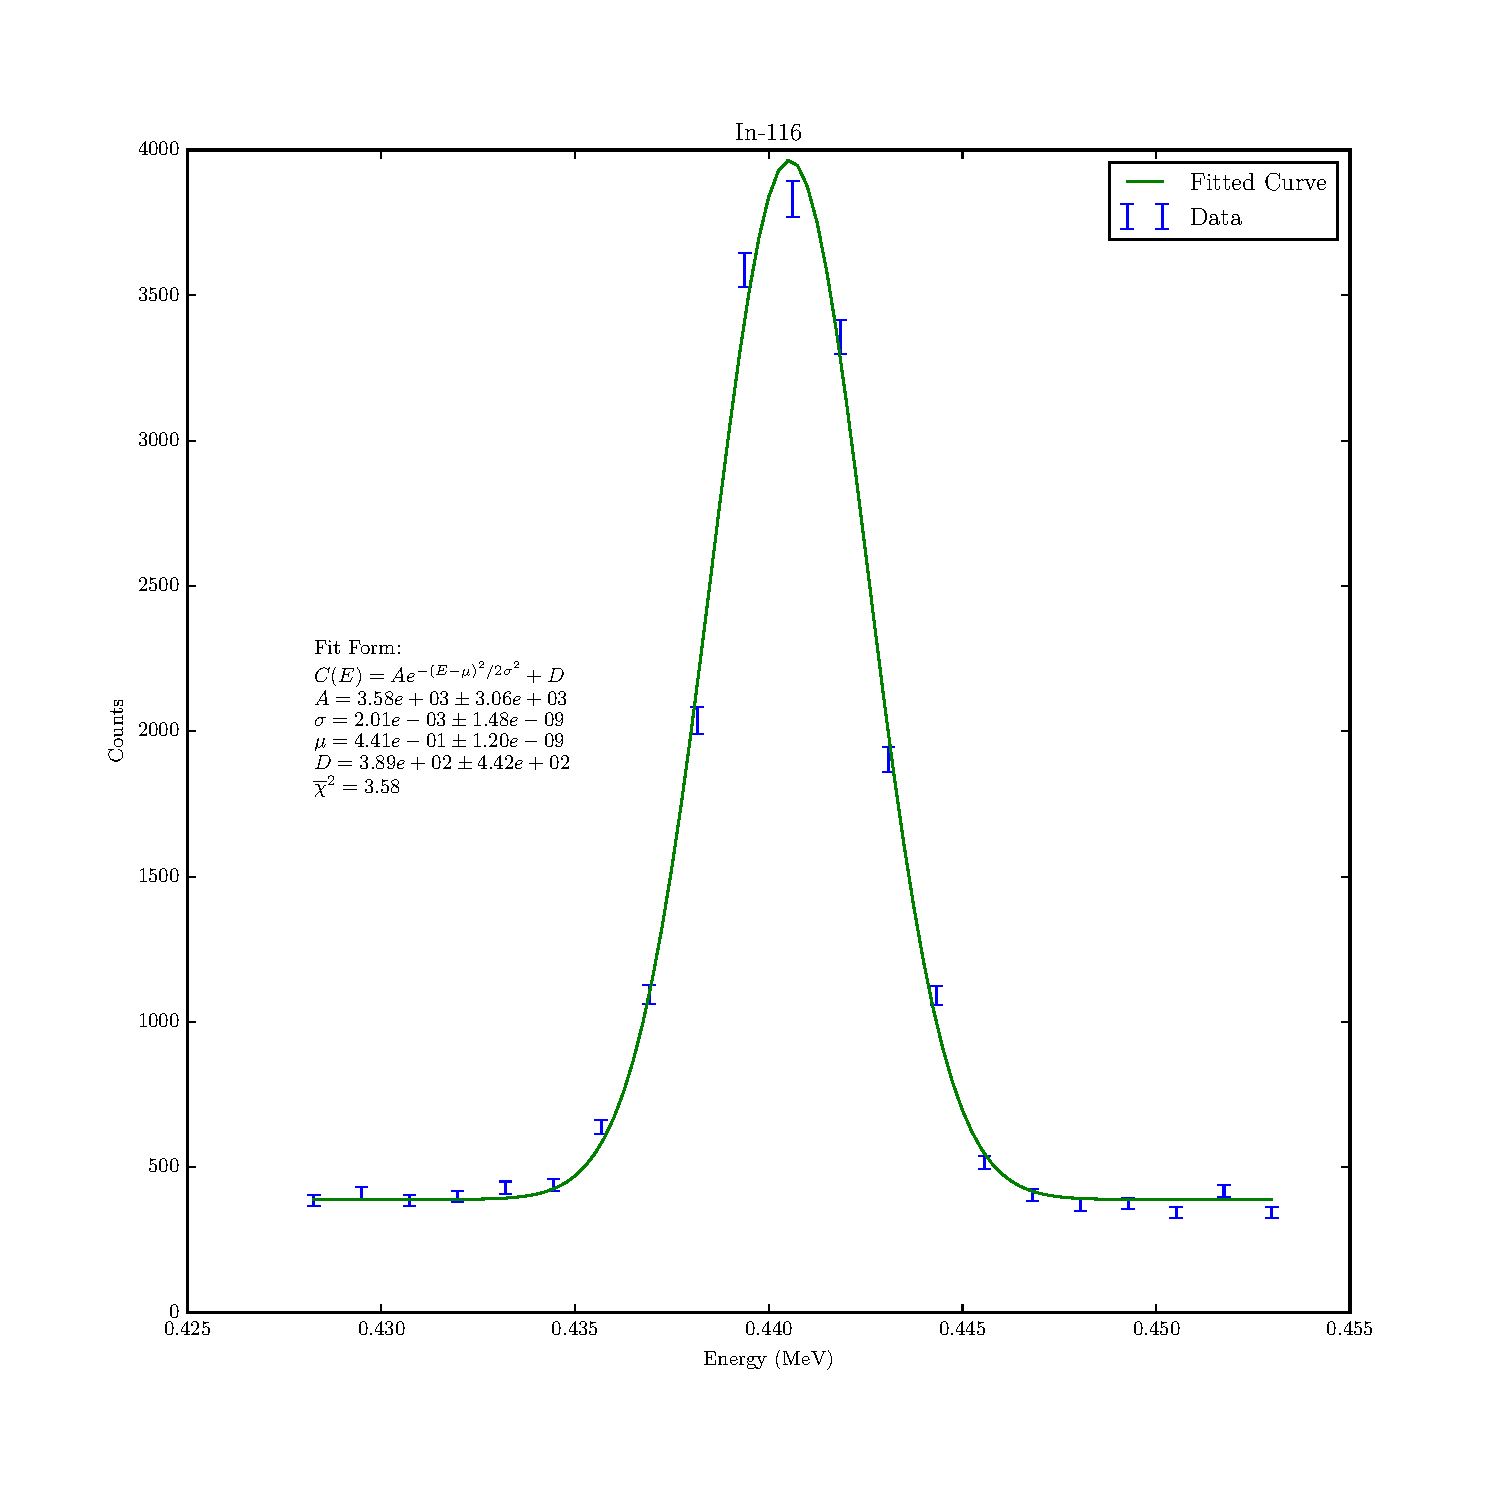
\includegraphics[width=\linewidth]{../plots/In-116_0_4405.pdf}
        \caption{One of the better examples of peaks, once fitted.  This confirms that our estimates for peak centers were accurate, and our estimation that the uncertainties were around 1 channel were also accurate. \label{fig:fitted_in}}
      \end{figure}

      Now that we have presented these lovely figures, we will summarize the results.  The following have been used for the analysis, while Table~\ref{tab:calibration_points} summarized the peaks used for calibration.

      \begin{table}[h]
        \centering
        \begin{tabular}{|c|c|}
          \hline
          T ($\pm 0.040$ MeV) & E ($\pm 0.036$ MeV) \\ \hline
          % T = [ 0.23294209  0.25148492  0.28238964  0.35532477  0.4183704   0.49872266
          %   0.62234153  0.86957927  0.90048399  1.06118852  1.08591229]
          %
          % E = [ 0.37881236  0.4072447   0.44062179  0.52221025  0.59143681  0.6804424
          %   0.83743836  1.0735504   1.10074656  1.26763203  1.29482818]
          %
          % dT = [ 0.04009665  0.04009665  0.04009665  0.04009665  0.04009665  0.04009665
          %   0.04009665  0.04009665  0.04009665  0.04009665  0.04009665]
          %
          % dE = [ 0.03638809  0.03638809  0.03638809  0.03638809  0.03638809  0.03638809
          %   0.03638809  0.03638809  0.03638809  0.03638809  0.03638809]

          0.233 & 0.378 \\ \hline
          0.251 & 0.407 \\ \hline
          0.282 & 0.441 \\ \hline
          0.355 & 0.522 \\ \hline
          0.418 & 0.591 \\ \hline
          0.499 & 0.680 \\ \hline
          0.622 & 0.837 \\ \hline
          0.870 & 1.074 \\ \hline
          0.900 & 1.101 \\ \hline
          1.061 & 1.268 \\ \hline
          1.086 & 1.295 \\ \hline
        \end{tabular}
        \caption{The reader will notice that the uncertainty in each energy and the uncertainty in each compton edge is roughly the same.  This is because we were able to estimate the location of each peak to within one channel and the location of the compton edges to within four channels in every case, and then simply performed the conversion from channels to energy.  Of course in both cases the uncertainty in the conversion is the same and that has of course been added as well. \label{tab:analysis_points}}
      \end{table}

      So now it would seem that we have everything together.  We've established our calibration, we've worked out how to propagate uncertainties through the conversion, and we've developed our table of peaks with corresponding compton edges to perform our analysis.

    \subsection{$\frac{p^2c^2}{2T} = BT + C$ - Relativistic Mass}
      We will now return to equation~\ref{eq:rel_mass} and equation~\ref{eq:fitfn}.  We can plot the quantity $\frac{p^2c^2}{2T}$, which we expect, classically to be the rest mass of the electron - and thus a constant.  This is not true in our case as we can see in Figure~\ref{fig:mnr}, we actually see a linear relation as we would expect from the relativistic relation, equation~\ref{eq:rel_dispersion}.  We can then rearrange eq~\ref{eq:rel_dispersion} and find the well-known relativistic dispersion relation by simply multiplying through by $2T$, whereupon we find:

      \begin{equation}
        p^2c^2 = 2m_ec^2T + T^2
      \end{equation}

      Notice that in the limit where $T << 2m_ec^2$, we recover the classical relation $p^2 = 2m_eT$.  This form thus successfully passes the common-sense tests that we use to make sure we are on the right track.

      \hspace{.25cm}

      Another feature that we should notice is the disparity between the line that we should have been clustered around had the calculated mass been exactly equal to the electron's rest mass of 511 keV, though it is within uncertainties.  We think that it's because we are working in a crystal, and so this value somehow represents an effective band mass, though this is not enirely clear and requires more in-depth experimentation and research.  One thing that we will notice quite immediately is that we can, in fact, extract the electron's rest mass (or, as we suspect, a mix of this and a band effective mass) by performing the following calculation (eq~\ref{eq:rest_mass}) - we will then take an average weighted by the uncertainty in each point and show the average.  This is best summarized in a plot, see Figure~\ref{fig:mass_avg}.  Now, the uncertainties are rather large - this is again due to inaccuracy in determining the compton edge energy perfectly.  We had an uncertainty of four channels in each determination of the compton edge which even as a fractional uncertainty dominates any other sources of error.

       \hspace{.25cm}

       We can calculate the electron's speed, which will be of use shortly in order to show other quantities of interest.  In this vein, we use equation~\ref{eq:velocity} with uncertainty given by equation~\ref{eq:dvelocity}.  These will give us our x axis and x uncertainty respectively when we plot the momentum as a function of velocity and the kinetic energy as a function of velocity going forward.

       \hspace{.25cm}

       Now we want to see if the relativistic form of the momentum (eq~\ref{eq:momentum}), holds in this case, that is, whether the lorentz factor is needed or not.  It turns out, of course, that it is, and the theoretical model fits the data quite well, as in Figure~\ref{fig:momvsspeed} .  Importantly - no actual fit was performed, only the model overlaid on the data points to give a rough inkling of what's going on.  In the same vein, we can find the relativistic expression for the kinetic energy in terms of the lorentz gamma, equation~\ref{eq:ke}, and plot the results as in Figure~\ref{fig:energyvsspeed}.  We find that the forms that take into account the proper lorentz gamma factors are in fact the proper forms, and that these electrons are most certainly going at significant fractions of $c$.

       \hspace{.25cm}

       Finally, we are going to plot the special relativistic dispersion relation, eq~\ref{eq:dispersion} as well as the classical dispersion relation along with our data points to see which one matches best.  Looking at Figure~\ref{fig:rel_dispersion}, it is fairly obvious that the relativistic form matches best, at values of $p$ corresponding to speeds in excess of $0.5c$ especially.  There is a small region for low $p$ where it is possible that either form fits, as we would expect - since special relativity reduces to classical mechanics in the $\beta << 1$ limit.  For the region with $\beta$ significant, we see that the band flattens - the electrons are behaving like photons rather than electrons and have a roughly linear band structure.

       \hspace{.25cm}

       Throughout, we have alluded to the fact that our uncertainties are dominated by the determination of the compton edge.  In general, we were unable to confidently identify the compton edge to within better than 4 channels, which is a huge fraction of our uncertainty values, and in fact makes the error from the calibration negligible and so we can ignore it (it is less than 0.01\% of the uncertainty in T).  There are many places where we likely overestimated how uncertain we were with our determination of the compton edges, but we were not comfortable assigning uncertainties based on how good the fits ended up, rather we decided that it is more correct to remain true to the original estimation and recognize that in the future more effort should be made to reduce these uncertainties - by either taking segmented sweeps or by focusing in more on one spectrum and finding the analytic expression for the compton edges, fitting them, and extracting the value that way.  The In-116 spectrum had an excellent array of edges and peaks and so we would likely focus on that.

    \section{Discussion of Results and Figures}
      In general we have demonstrated that the electrons knocked free by these photon scattering events are clearly in the regime where their velocity is a significant fraction of the speed of light, and thus can be considered to be relativistic.  This would incur further reading and research as to whether there are other effects that need to be taken into account - whether we have to deal with a band effective mass for the electron, as we suspect, and whether there is a bleeding of energy due to the fact that the local stress-energy tensor is no longer only in the mass portion.  These would likely be small-ish corrections however, and those concerns aside - it would seem as though the special relativistic regime works to explain the experimental phenomena quite well.

      \hspace{.25cm}

      We calculated a value for the electron's rest mass of $0.5003\pm0.0001$ MeV.  This was not within uncertainties of the literature value.  Our confidence that this exact value is true is not high because our uncertainties were so large, however.  We are unsure whether this is indicative of a systematic uncertainty in the energy calibration, which is possible and would cause all the mass points to shift down as we see they are shifted, or whether we are simply measuring a band effective mass, though the latter is unlikely.  Simply put, we're not sure why the mass is a little low, but it's probably due to some inaccuracies in the detector, gain, or calibration due to our inexperience with the device.  If we were to repeat the experiment we are confident that we would recover values that are much closer to the accepted literature, and if we didn't, then we would have convincing evidence that we are measuring the rest mass along with something else entirely.

      \hspace{.25cm}

      Another feature that is predicted by the theory of special relativity, if we reference figures~\ref{fig:momvsspeed} and~\ref{fig:energyvsspeed}, is the spiking of the energy and momentum as $\beta$ goes to 1.  This allows us to confirm the idea that it would take infinite energy to accelerate an object to the speed of light, and a feature which further follows many predictions of a light object traveling in a near-flat spacetime, most especially the divergence of the stress-energy tensor as we approach $\beta = 1$.

      \hspace{.25cm}

      The group that performed this experiment included me (Aman LaChapelle) and Sophia Kim.  We would like to thank the staff of the Advanced Undergraduate Physics Laboratory, especially Dave McCowan and Brian Mohs for answering our questions and taking the time to read all these words, respectively.

    \begin{widetext}

      \begin{figure}[h]
        \centering
        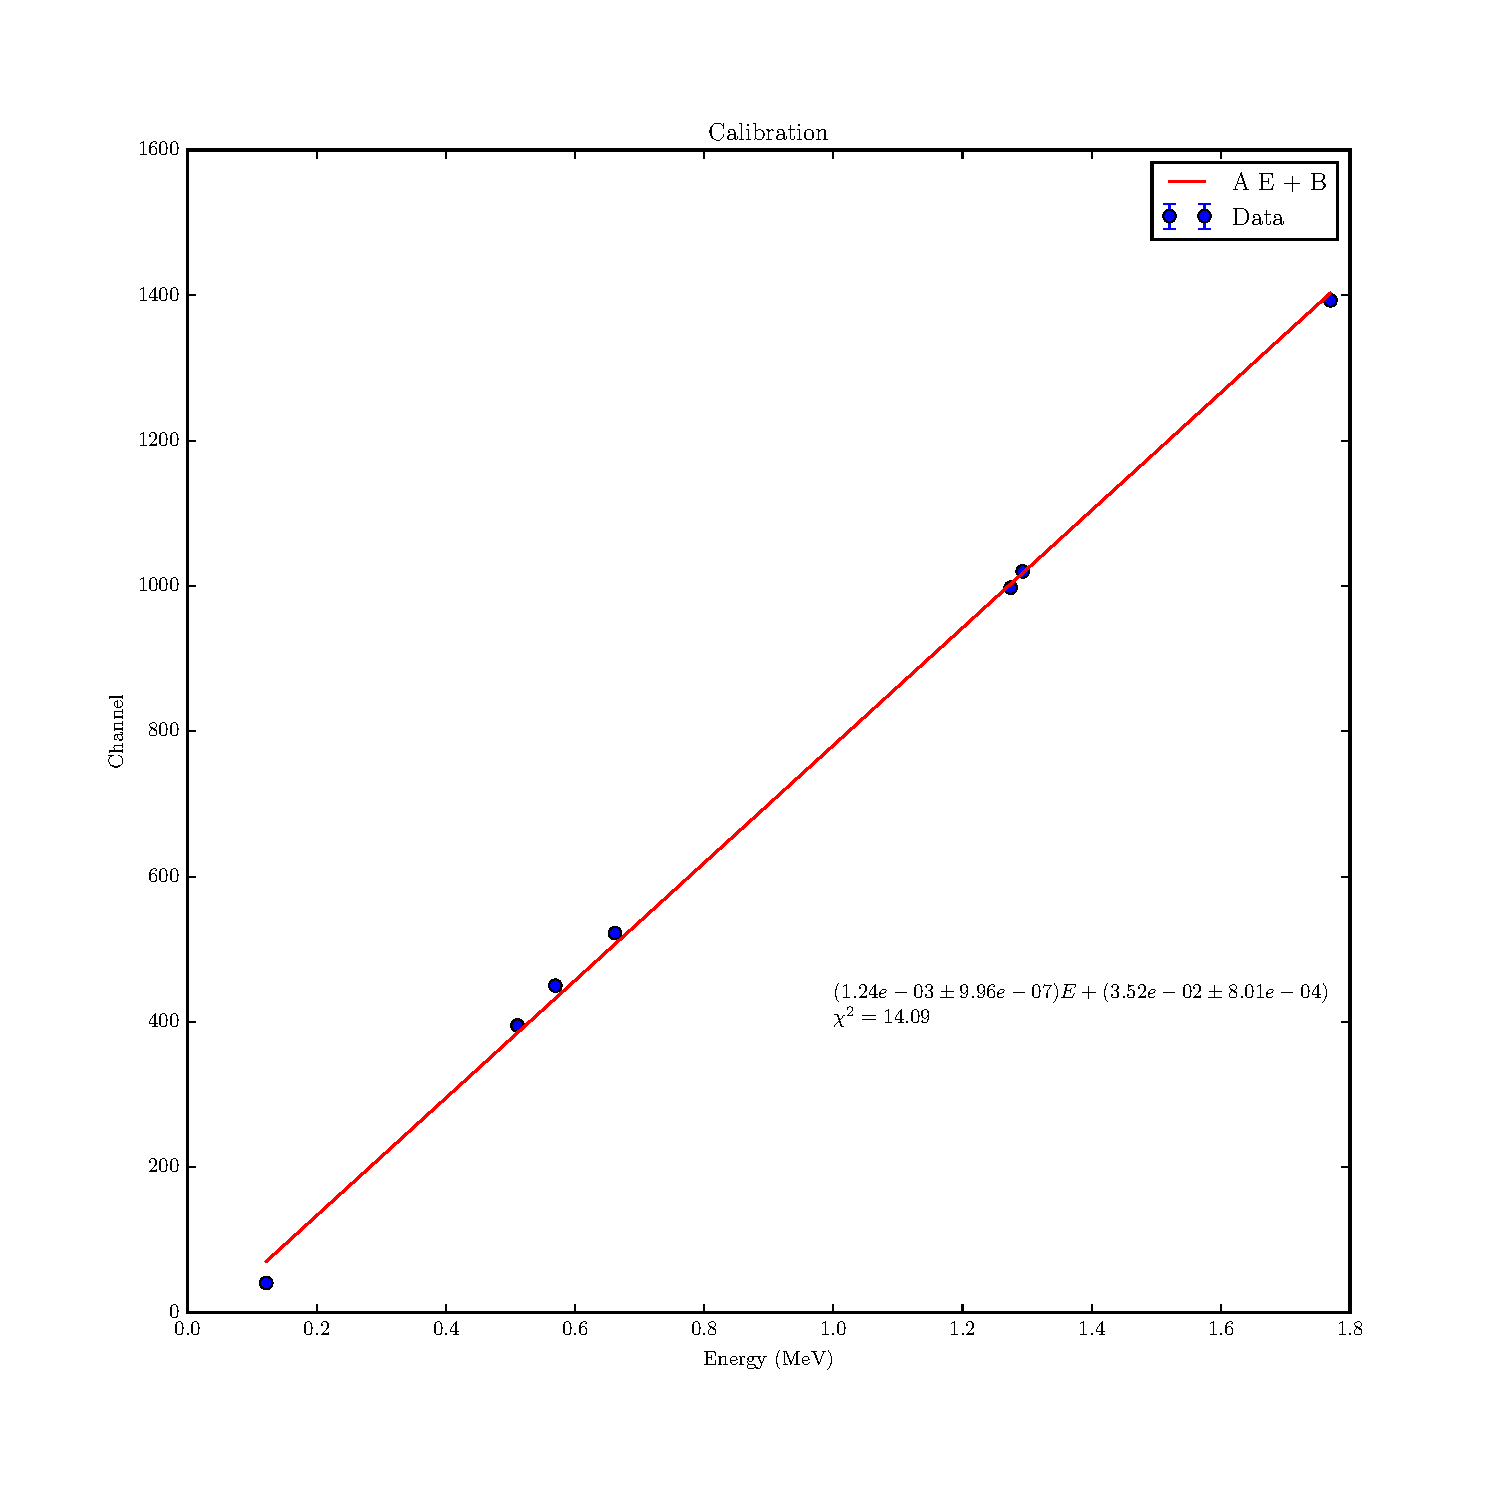
\includegraphics[width=\linewidth]{../plots/calibration.pdf}
        \caption{The point uncertainties are extraordinarily low because we are using full-energy peaks to get these points.  This means that they can be determined to around 1 channel, and as such uncertainties will be very small. \label{fig:calibration}}
      \end{figure}

      \begin{figure}[h]
        \centering
        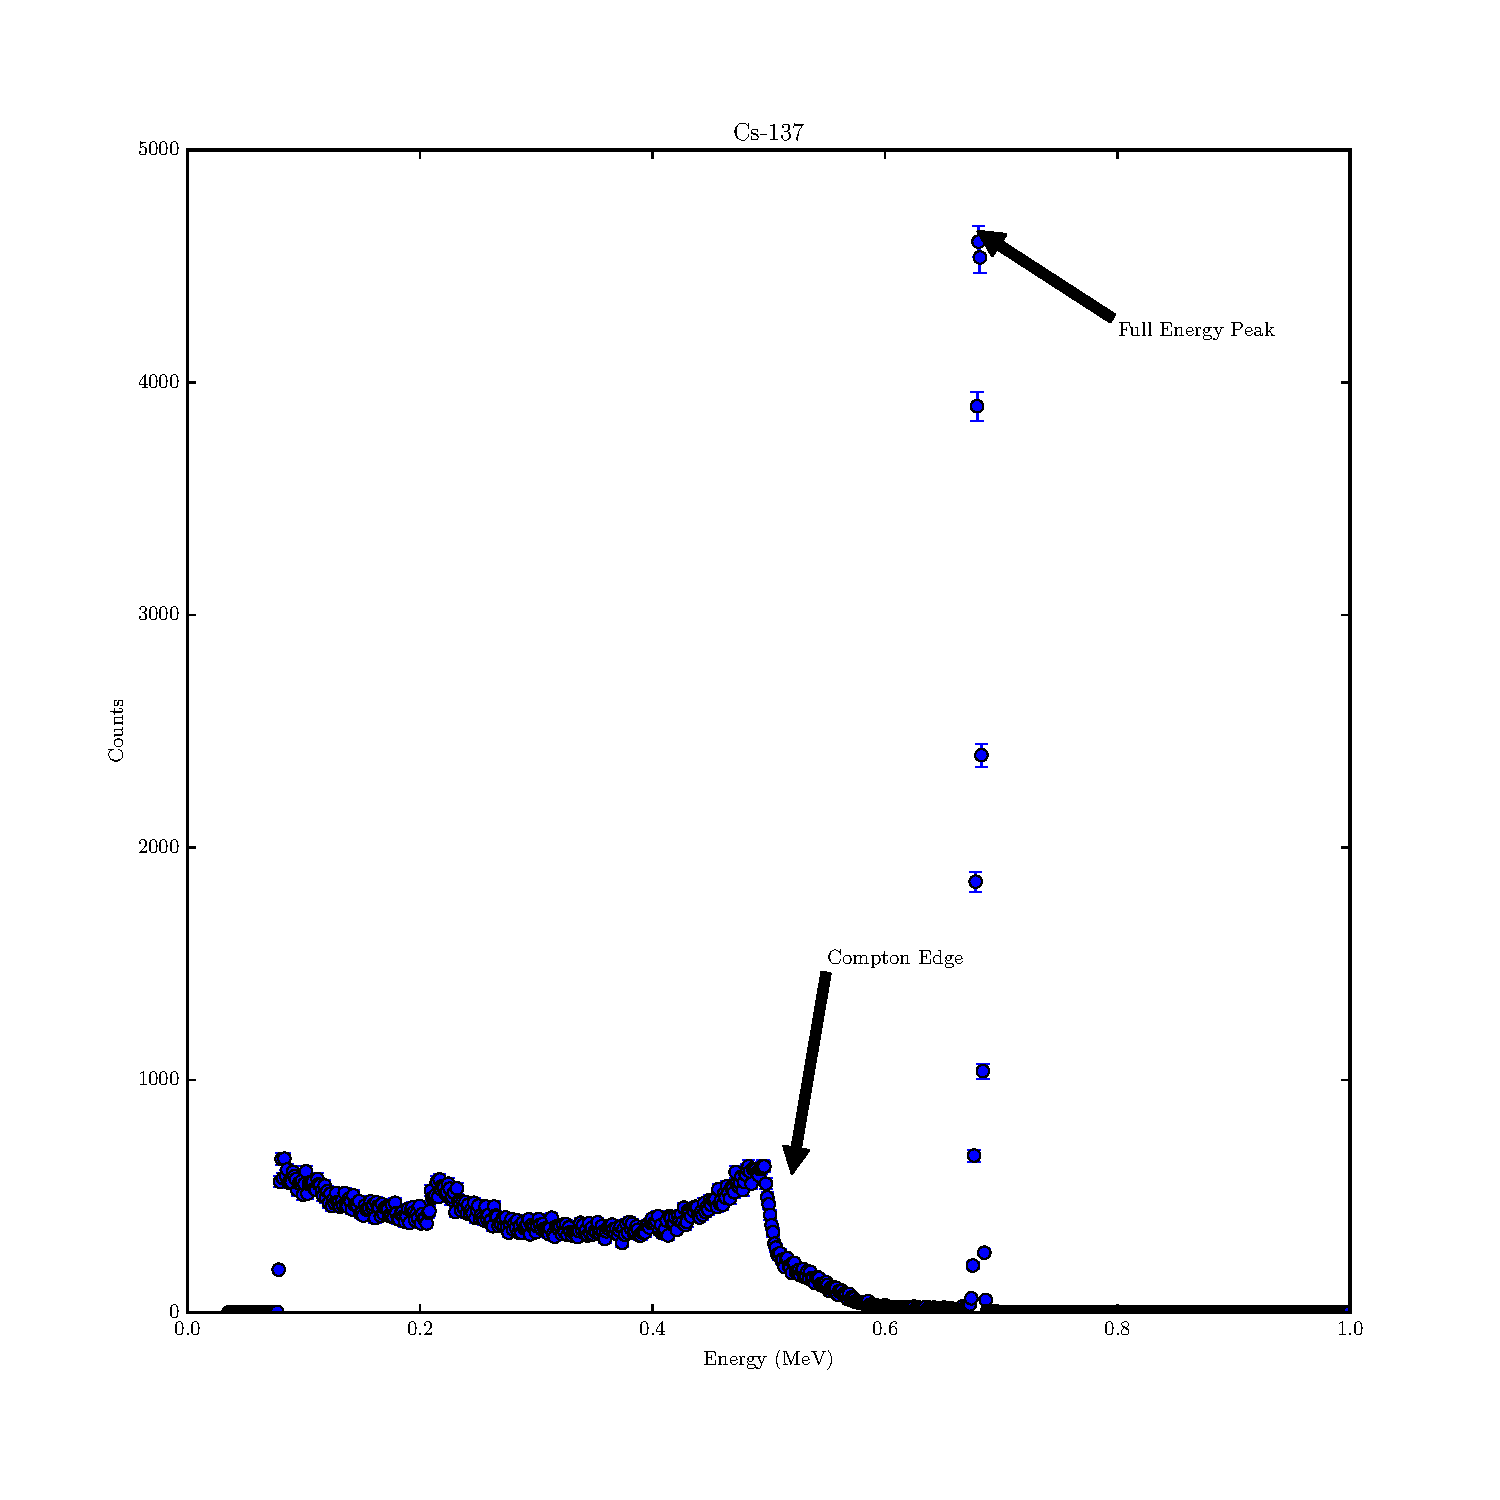
\includegraphics[width=\linewidth]{../plots/Cs-137.pdf}
        \caption{Cs-137 with full energy peak and Compton edge identified \label{fig:cs}}
      \end{figure}

      \begin{figure}[h]
        \centering
        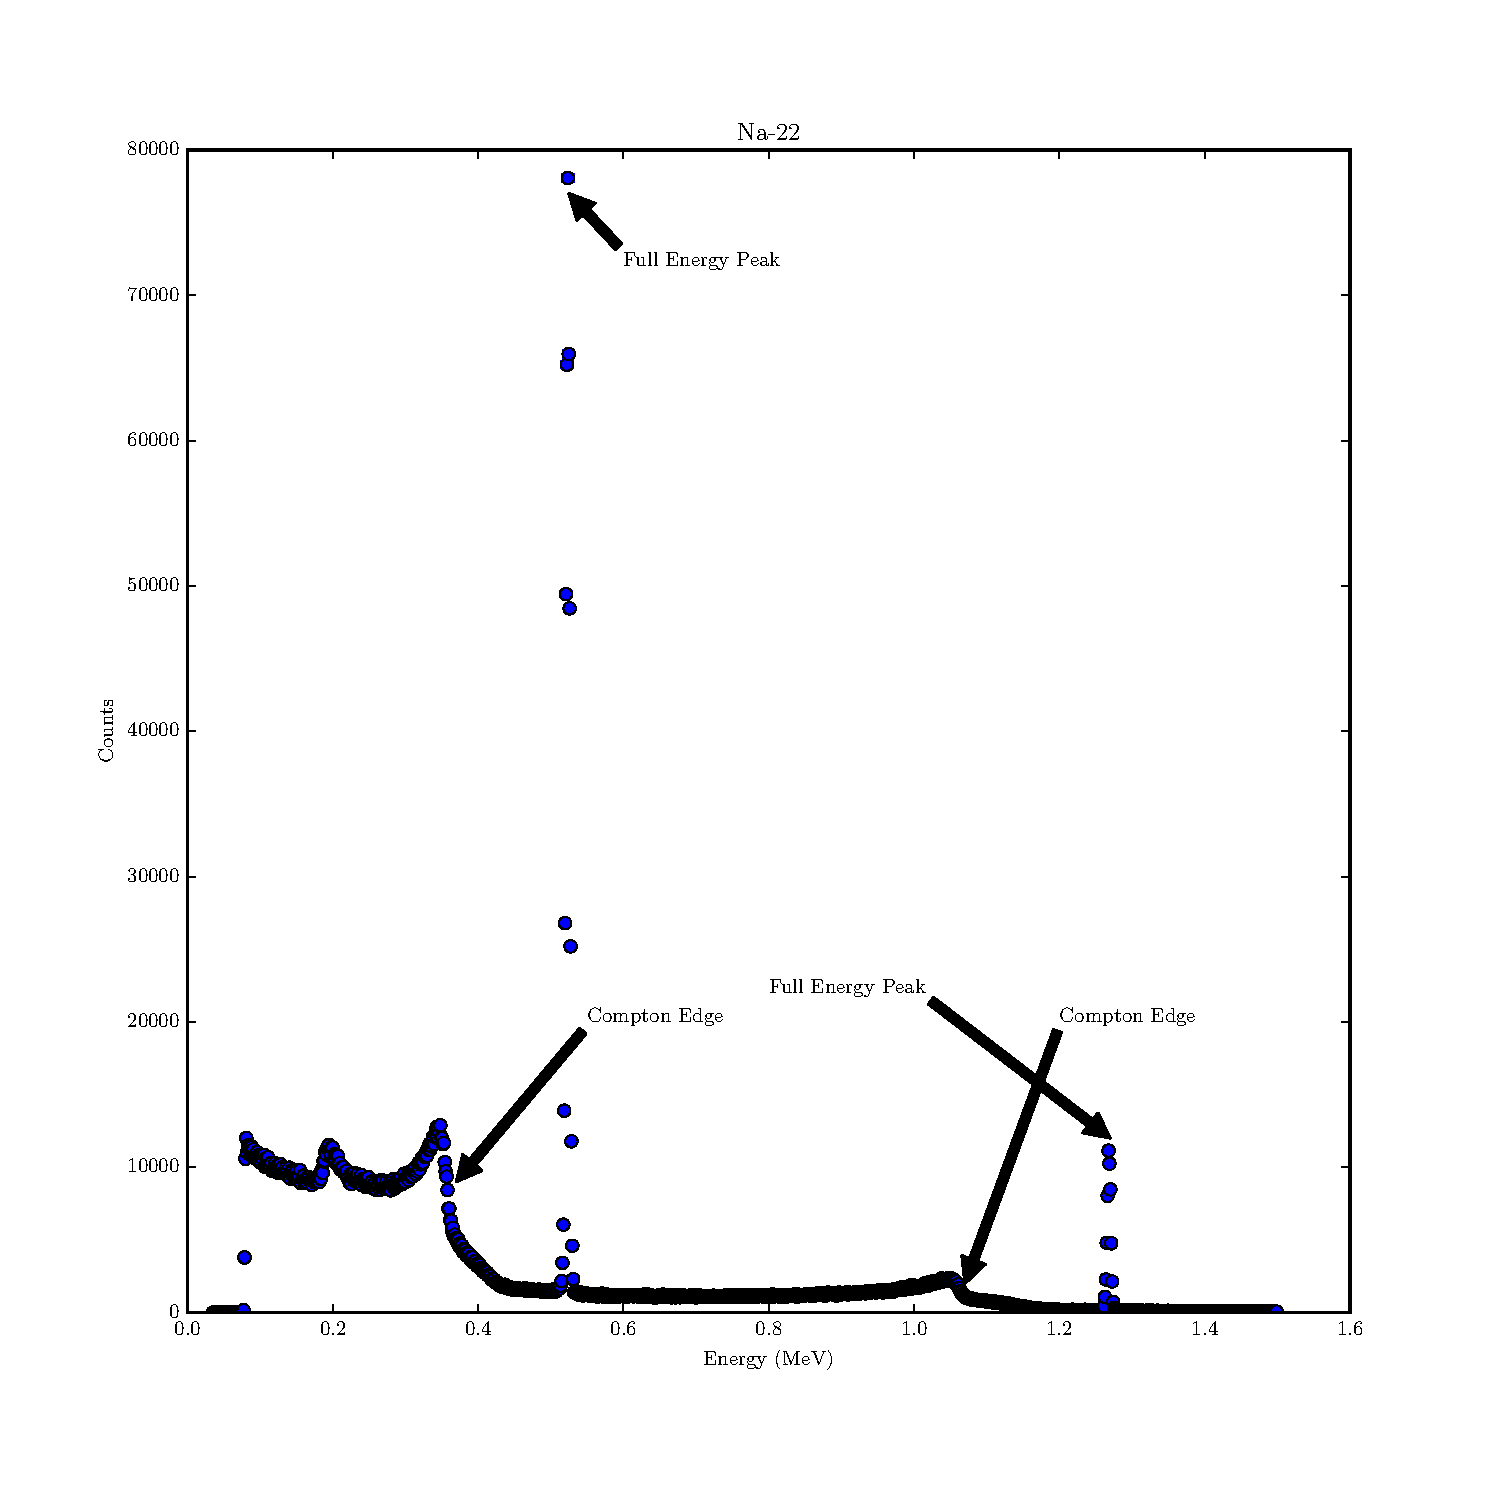
\includegraphics[width=\linewidth]{../plots/Na-22.pdf}
        \caption{Na-22 with full energy peaks and Compton edges identified \label{fig:na}}
      \end{figure}

      \begin{figure}[h]
        \centering
        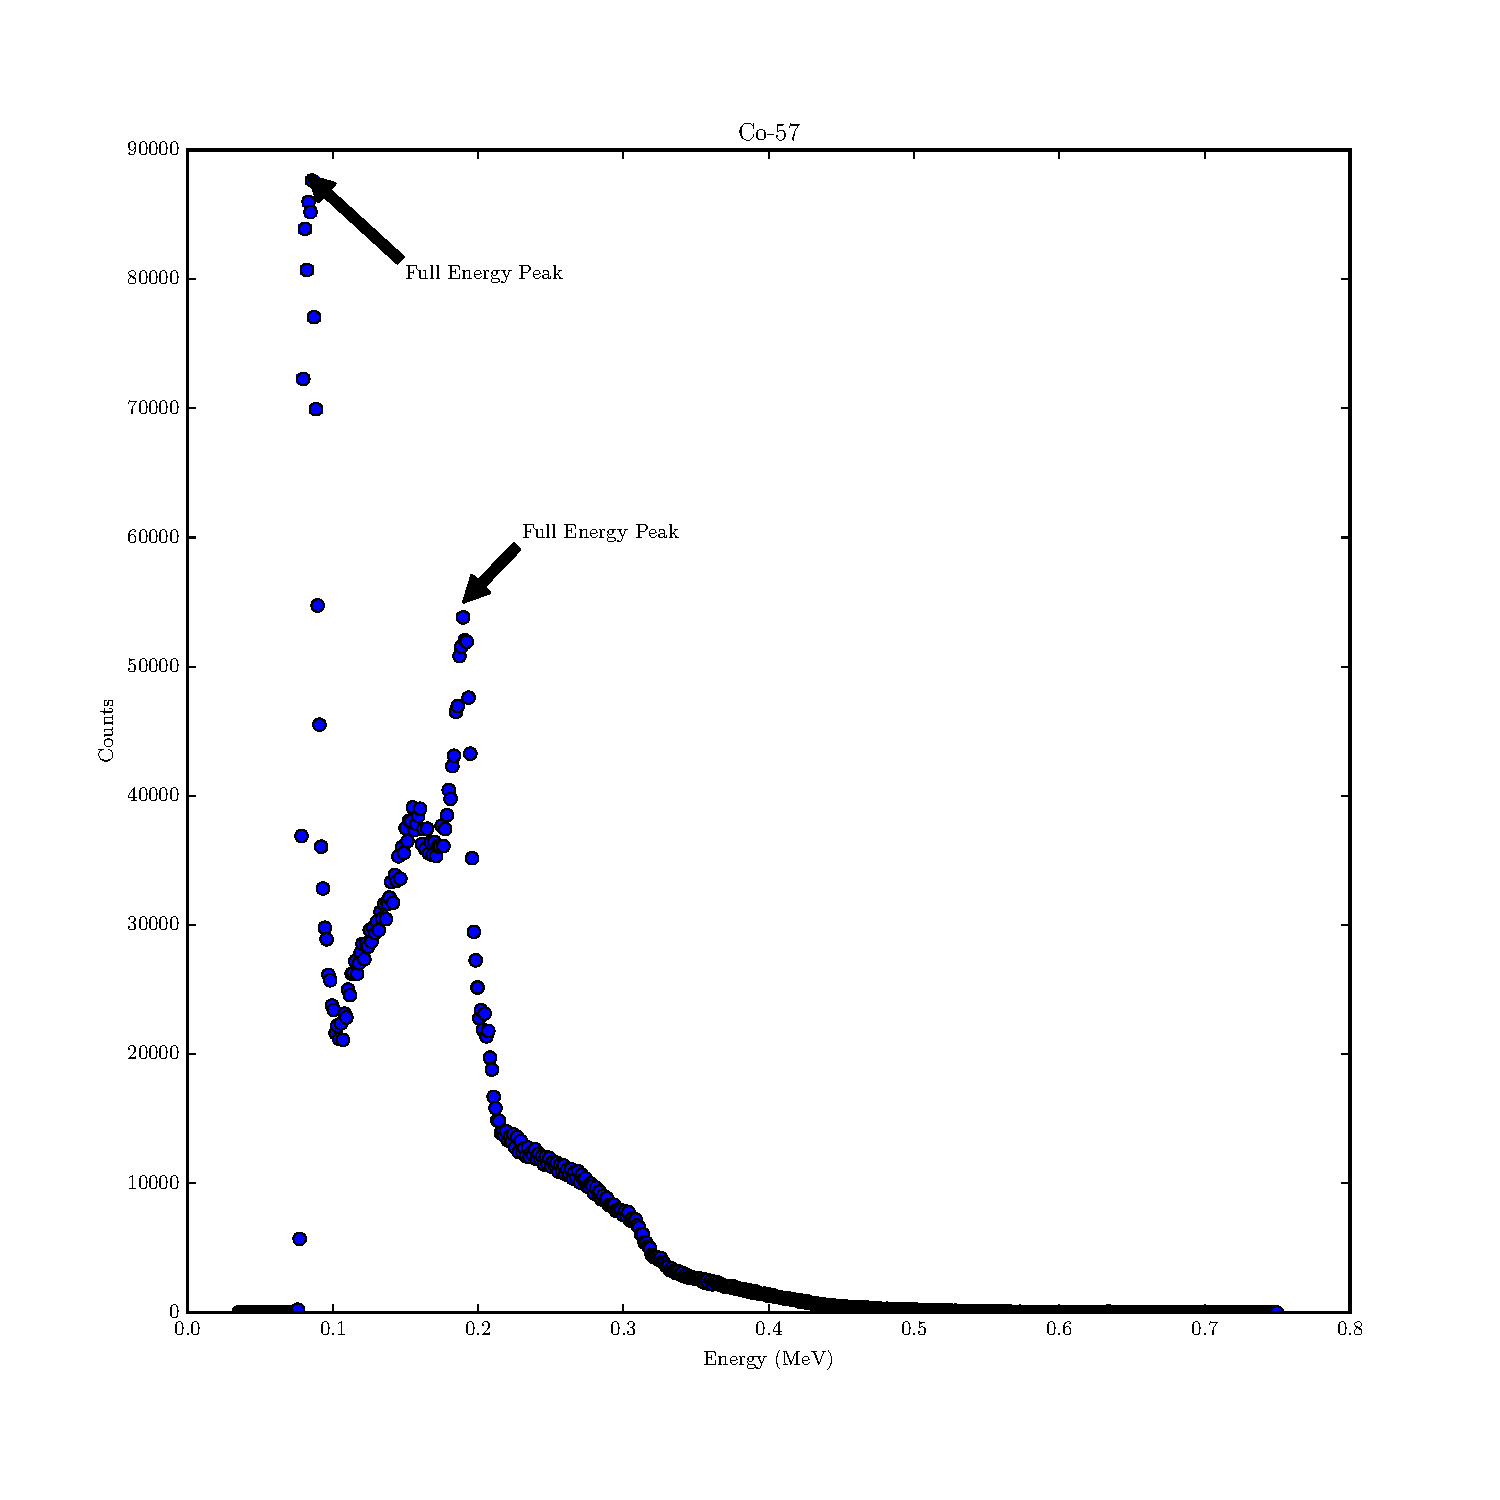
\includegraphics[width=\linewidth]{../plots/Co-57.pdf}
        \caption{Co-57 with full energy peaks identified \label{fig:co}}
      \end{figure}

      \begin{figure}[h]
        \centering
        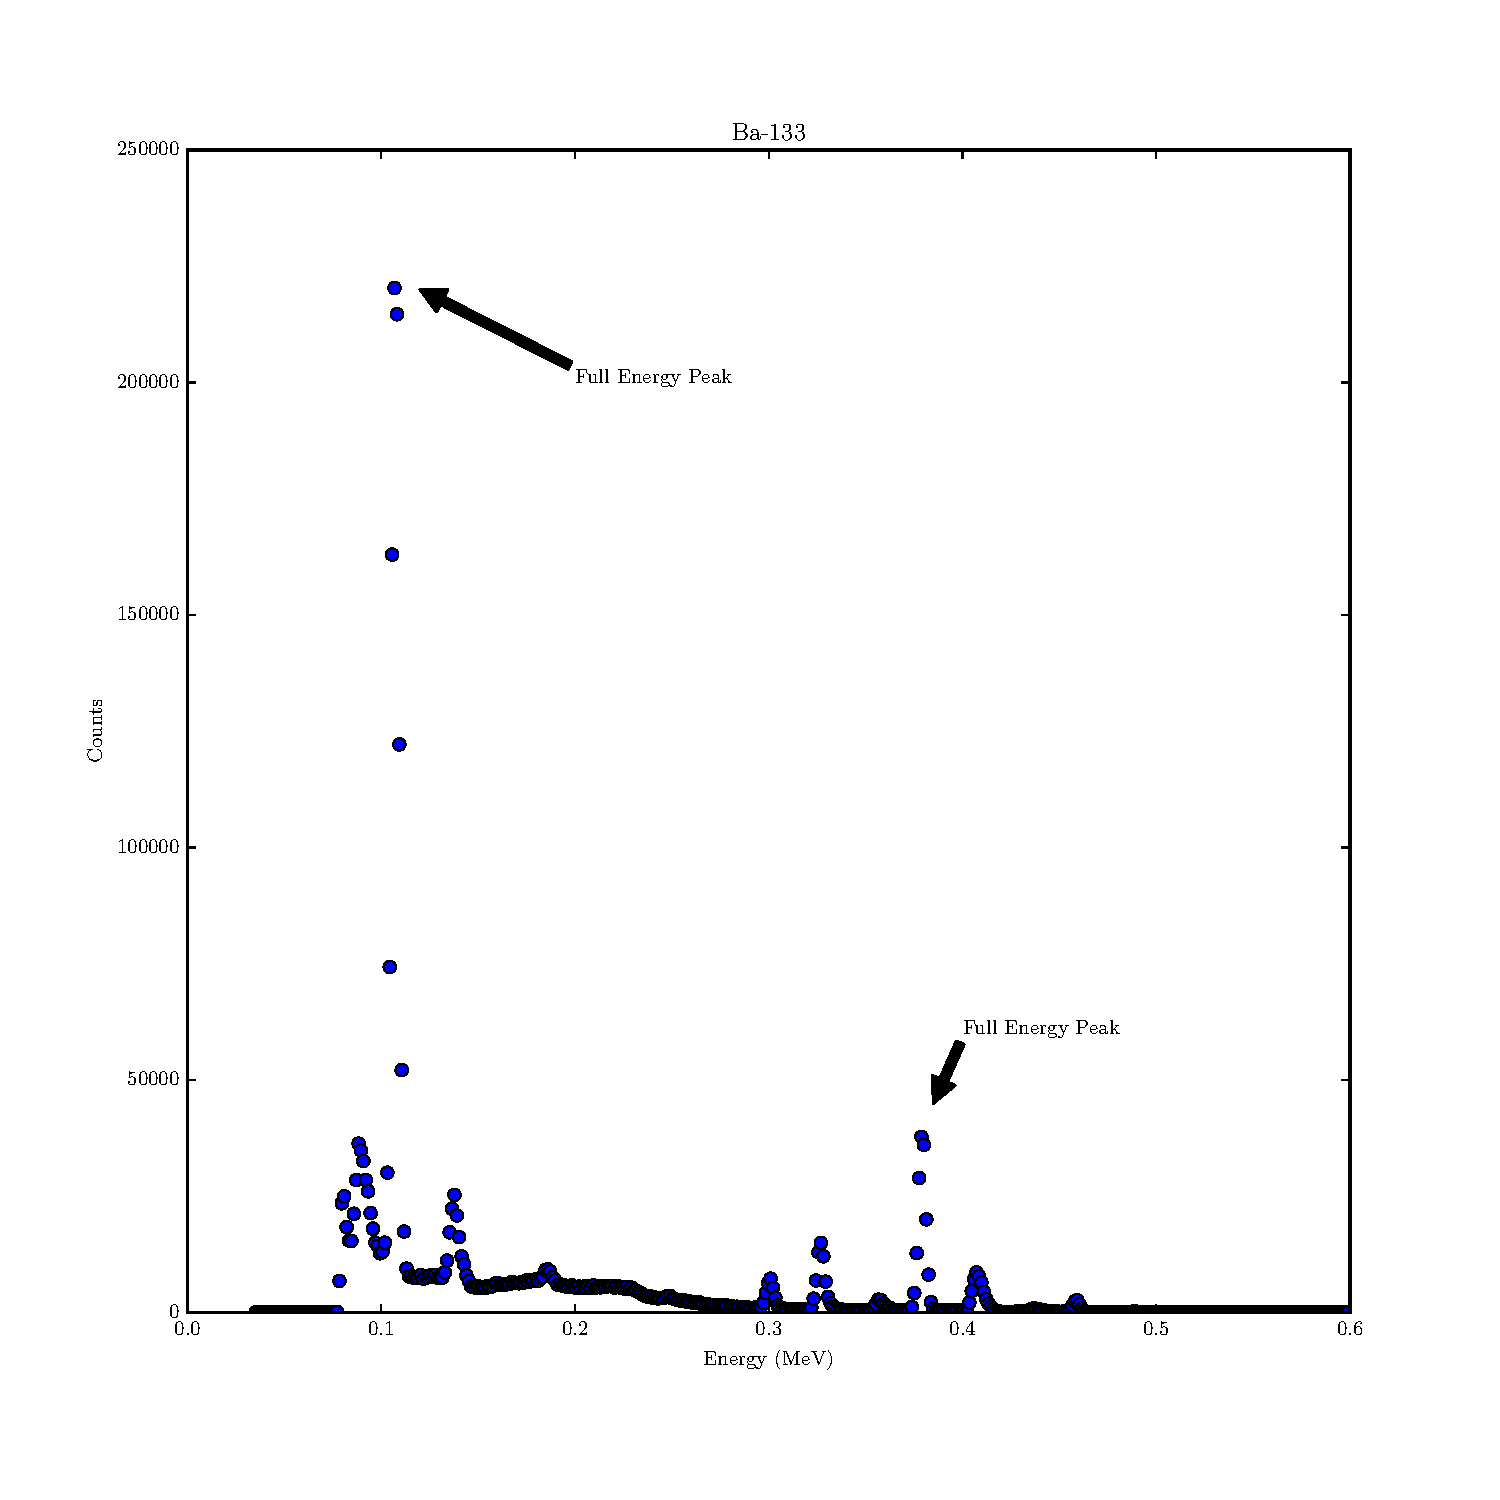
\includegraphics[width=\linewidth]{../plots/Ba-133.pdf}
        \caption{Ba-133 with full energy peaks identified \label{fig:ba}}
      \end{figure}

      \begin{figure}[h]
        \centering
        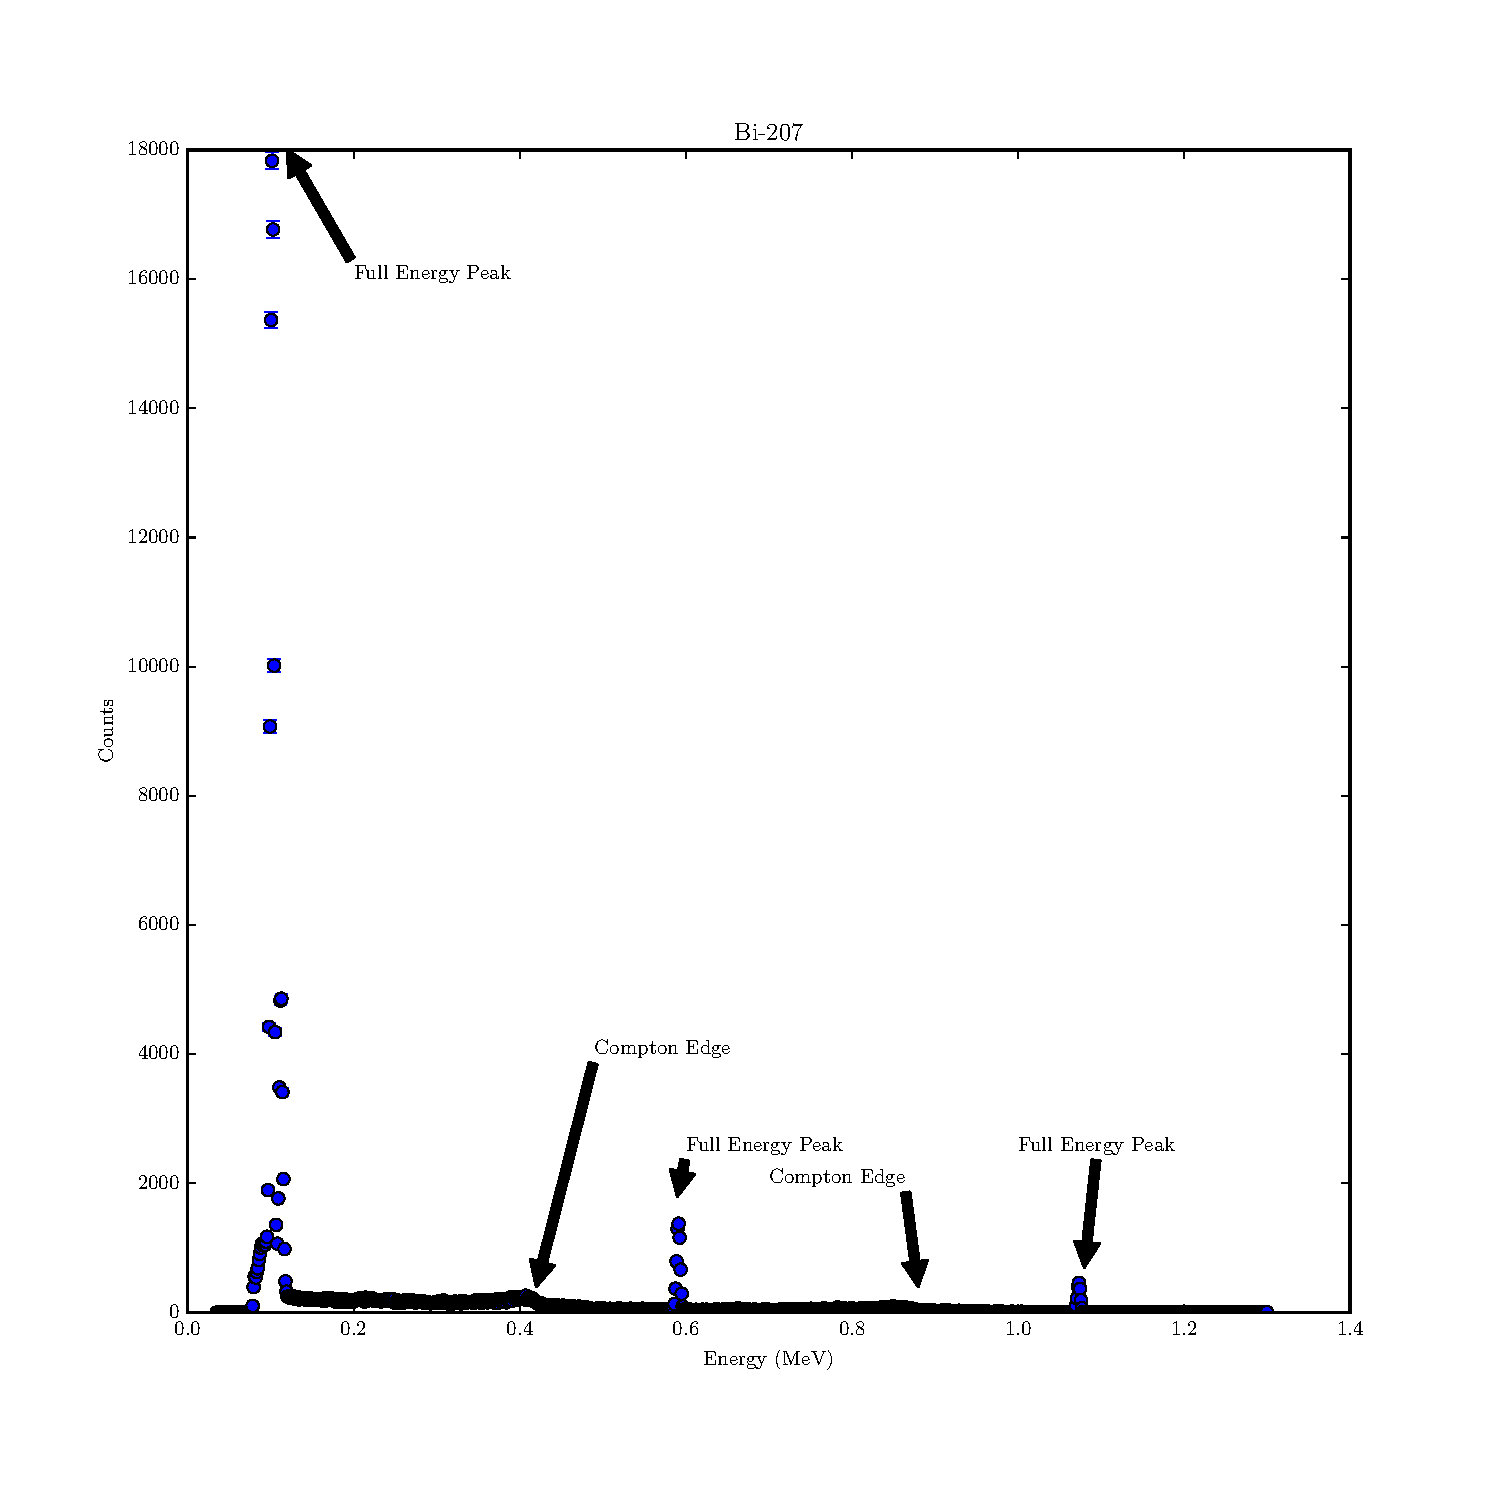
\includegraphics[width=\linewidth]{../plots/Bi-207.pdf}
        \caption{Bi-207 with full energy peaks and Compton edges identified \label{fig:bi}}
      \end{figure}

      \begin{figure}[h]
        \centering
        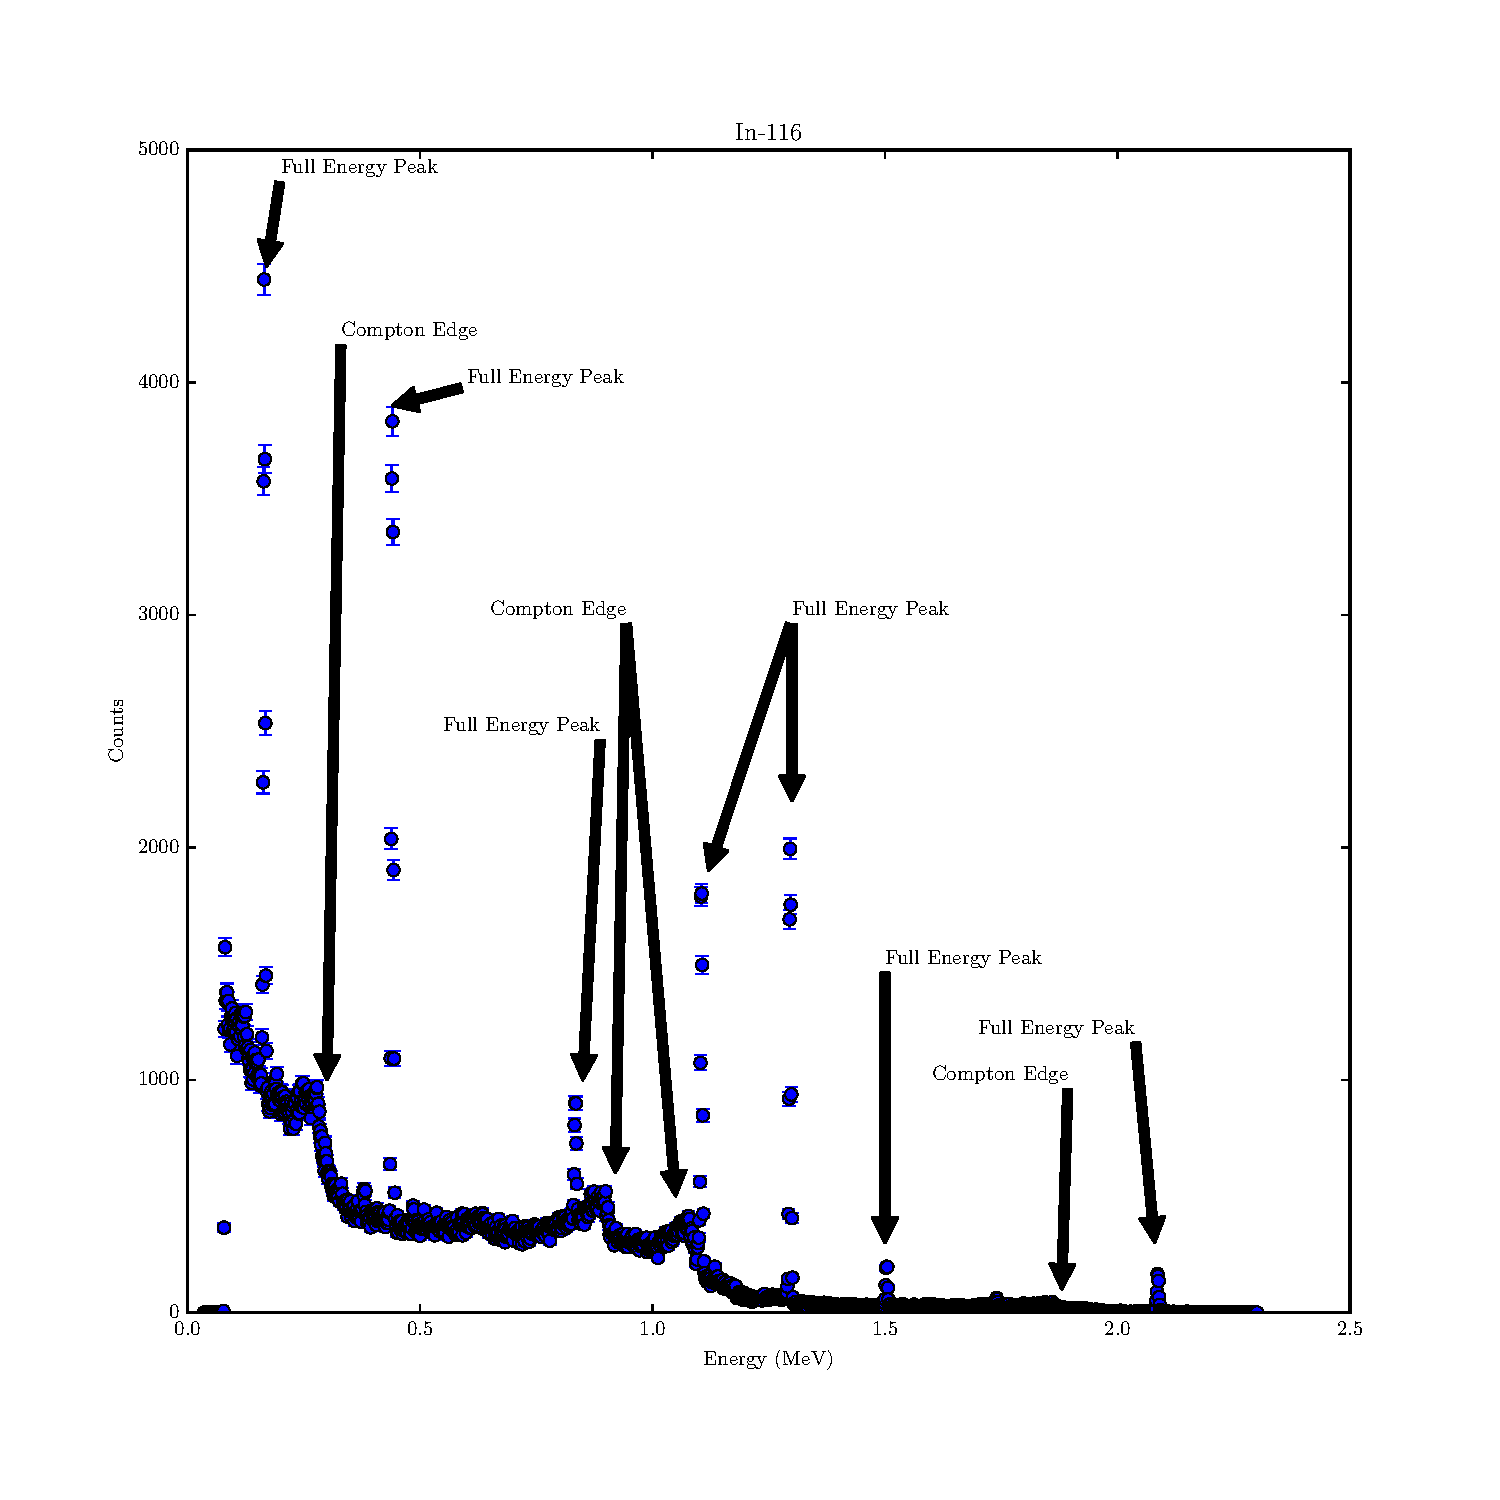
\includegraphics[width=\linewidth]{../plots/In-116.pdf}
        \caption{In-116 with full energy peaks and Compton edges identified \label{fig:in}}
      \end{figure}

      \begin{figure}[h]
        \centering
        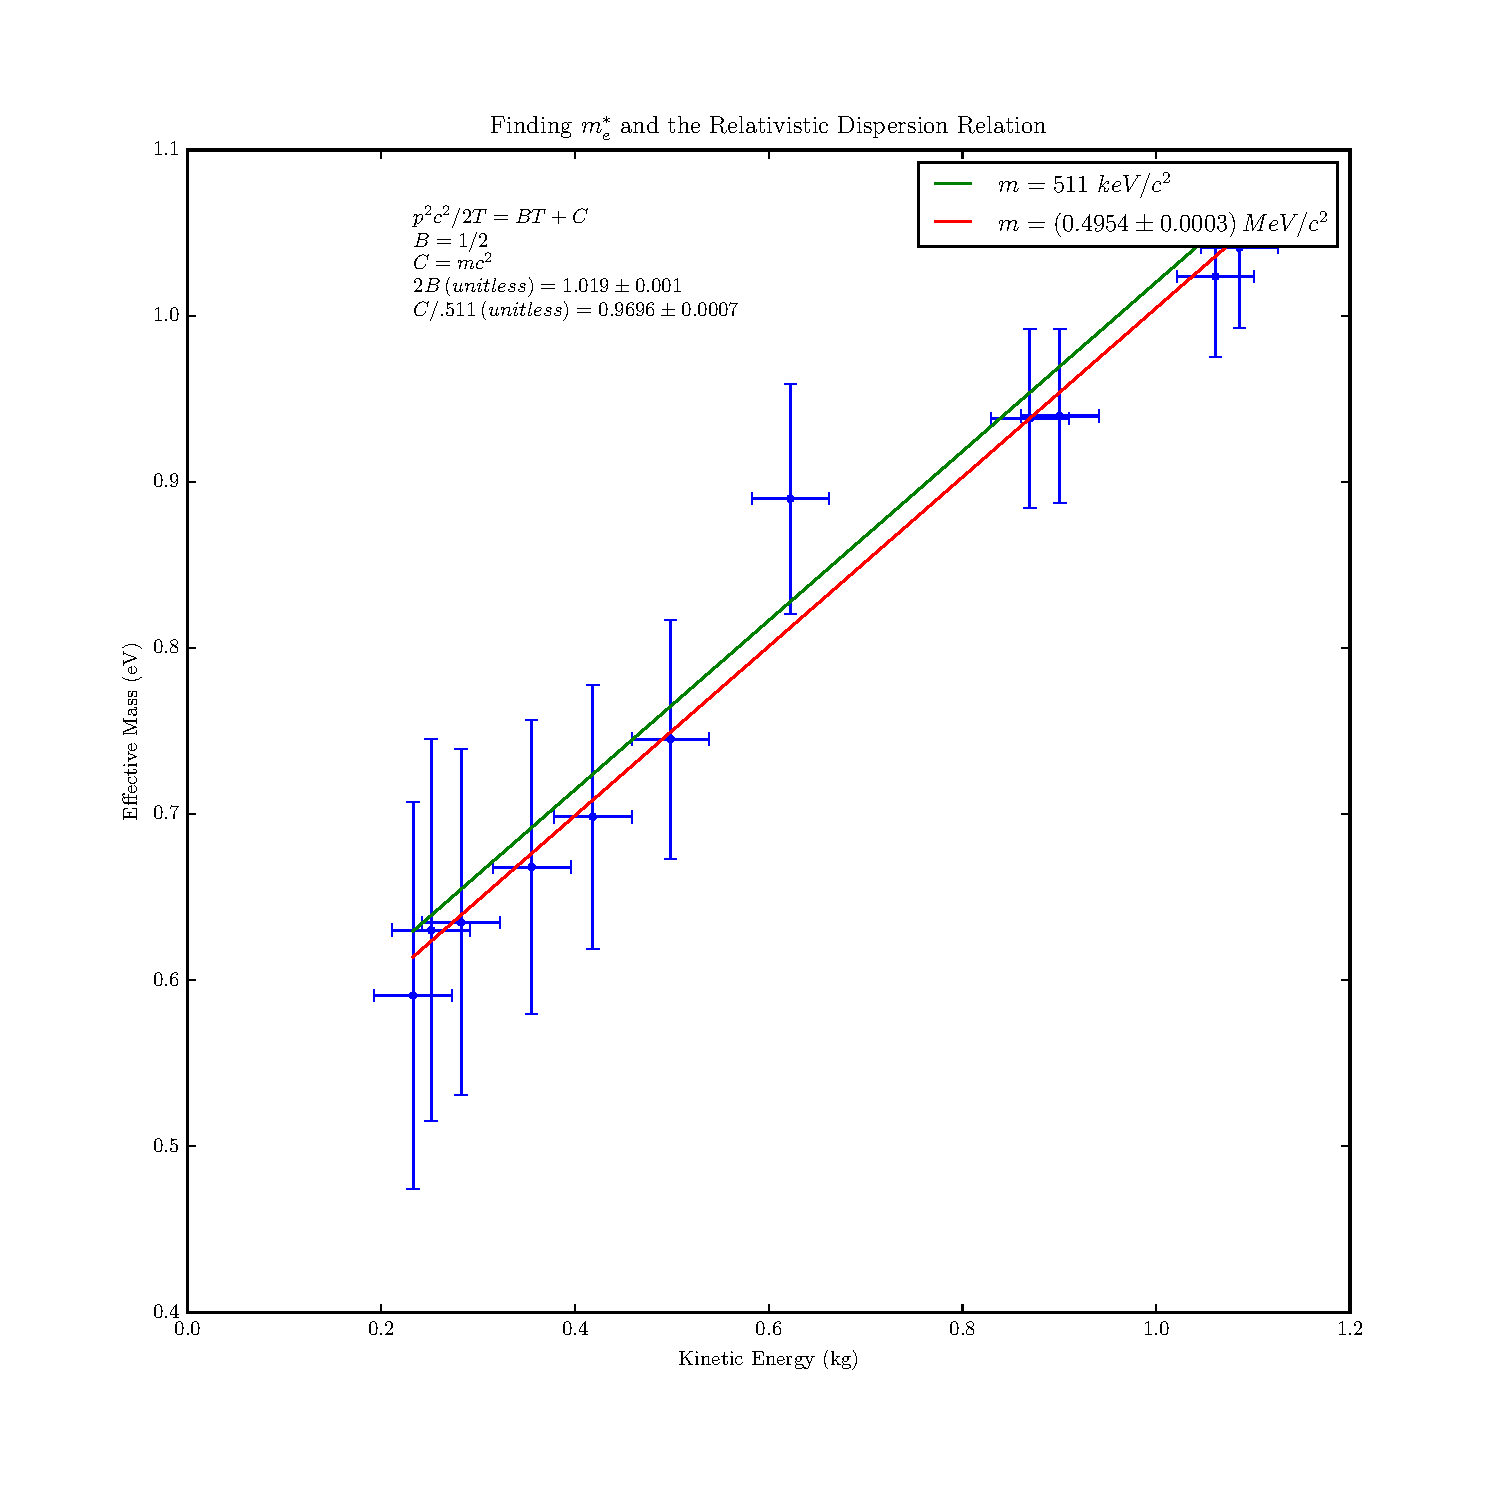
\includegraphics[width=\linewidth]{../plots/dispersion.pdf}
        \caption{A determination of the electron's rest energy and the relativistic dispersion relation. \label{fig:mnr}}
      \end{figure}

      \begin{figure}[h]
        \centering
        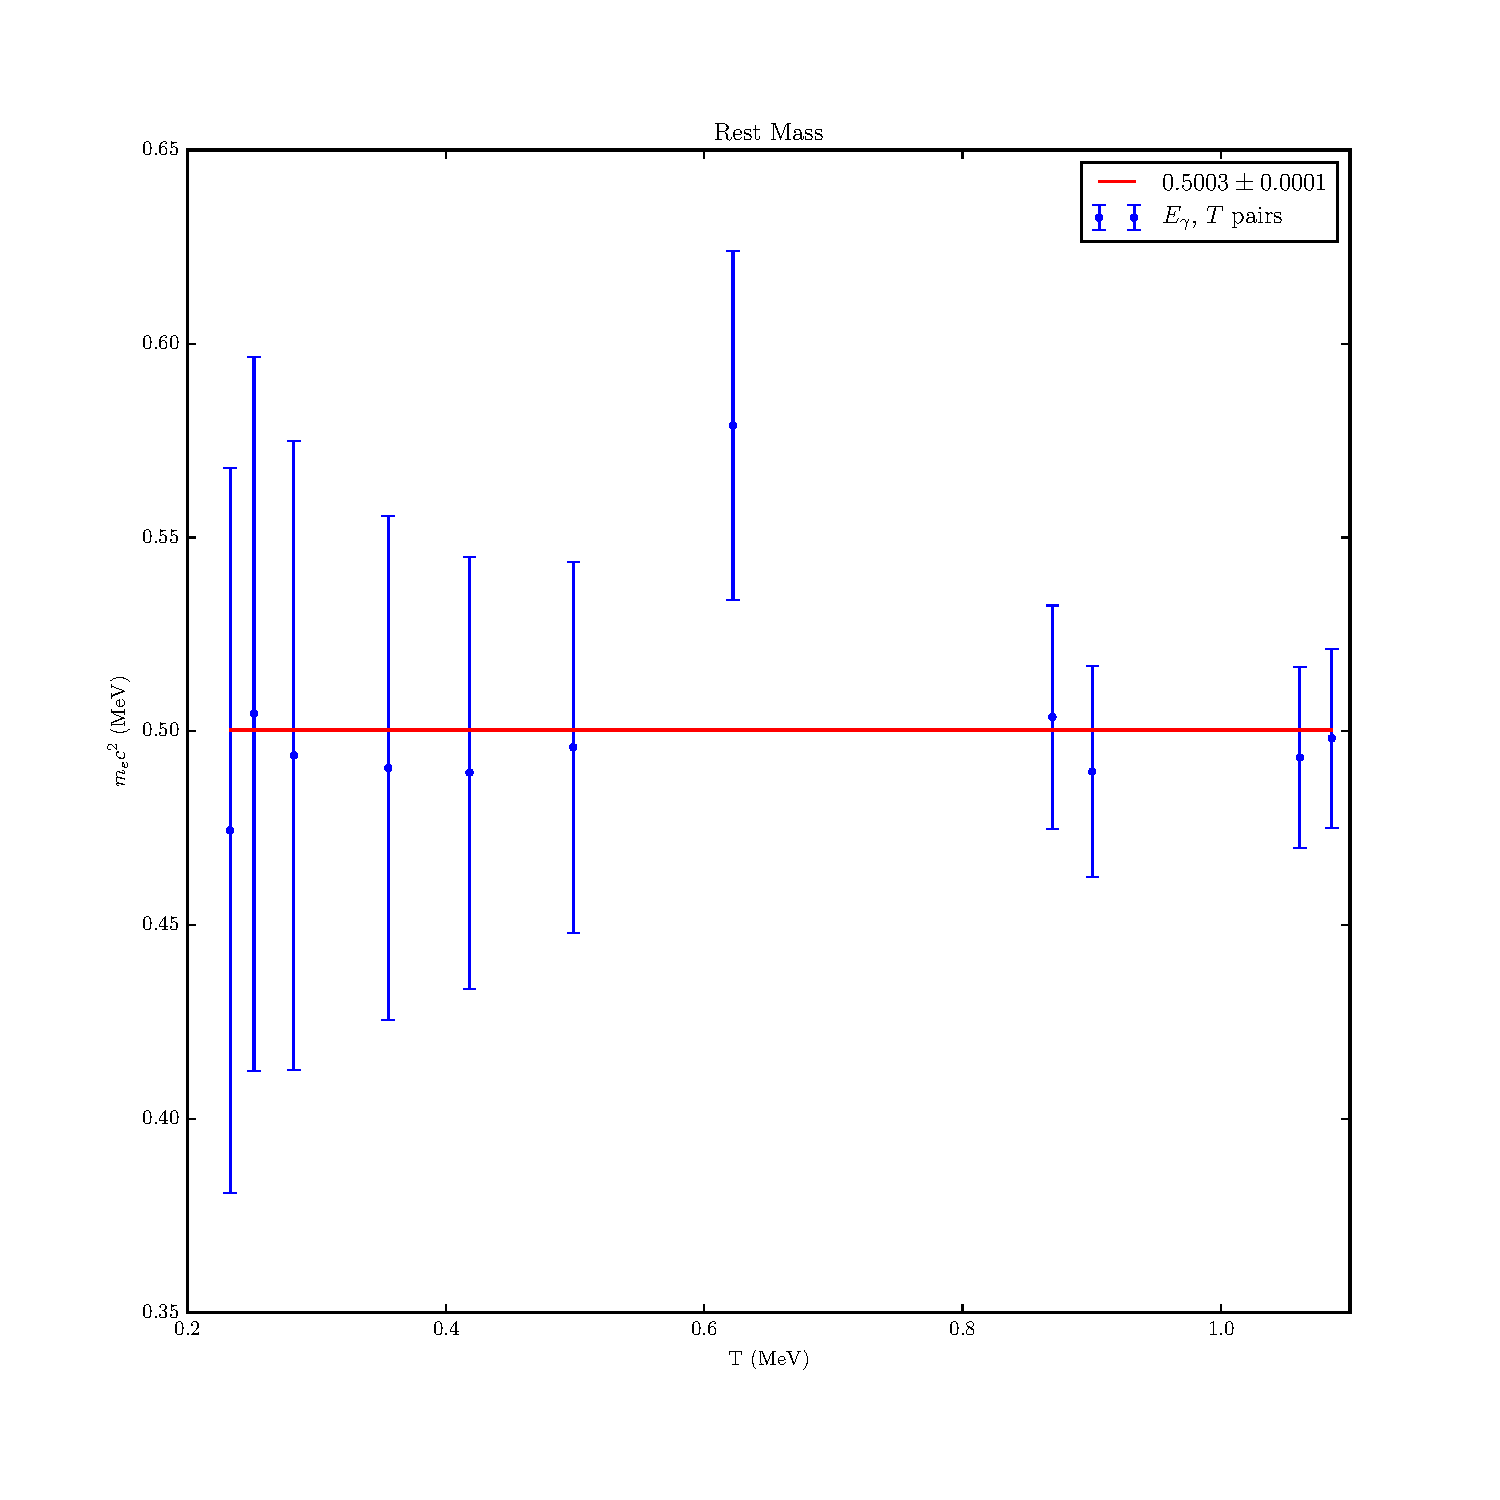
\includegraphics[width=\linewidth]{../plots/rest_mass.pdf}
        \caption{The electron's rest mass is found by averaging the rest mass found from each $E_\gamma$, $T$ pair and weighting by the uncertainty in each measurement. \label{fig:mass_avg}}
      \end{figure}

      \begin{figure}[h]
        \centering
        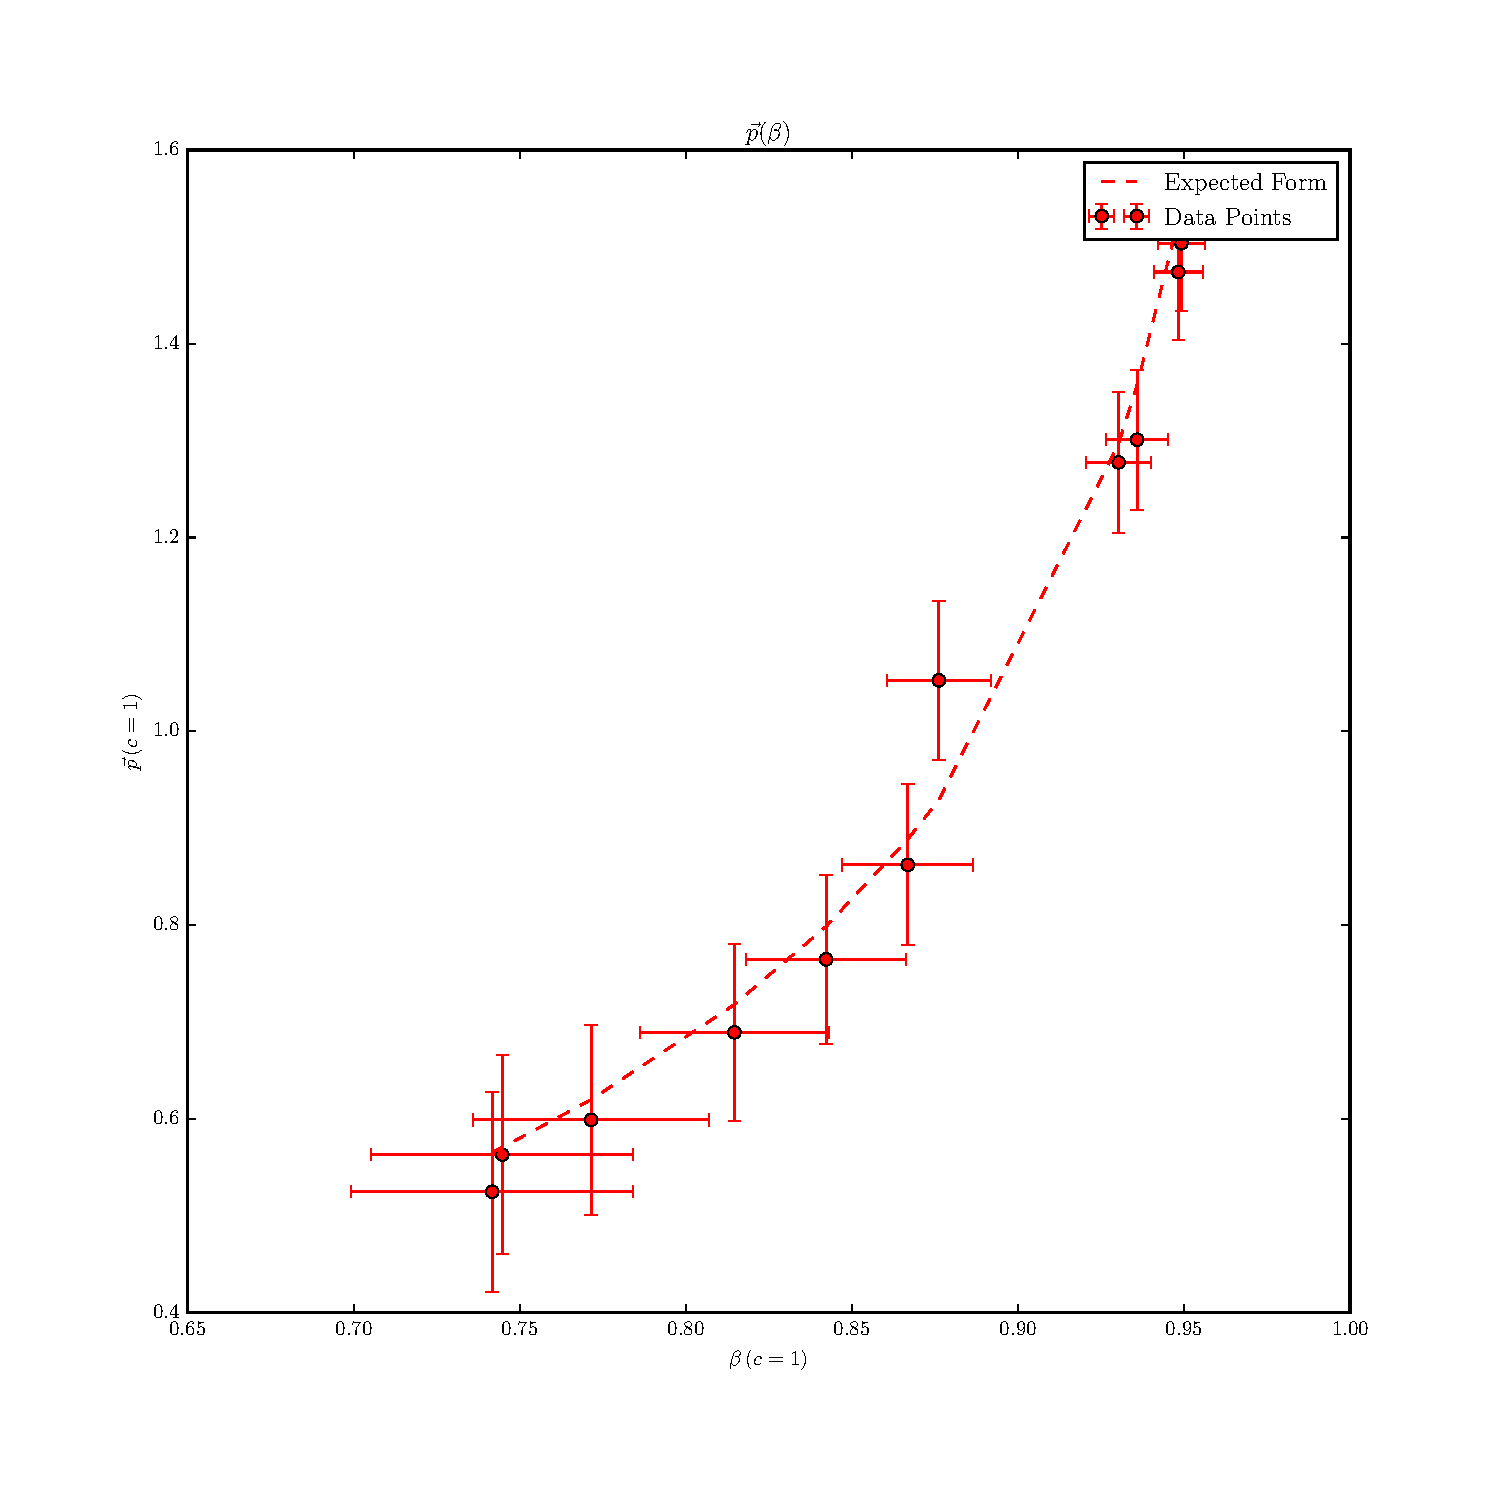
\includegraphics[width=\linewidth]{../plots/momvsspeed.pdf}
        \caption{The relativistic momentum expression is overlaid on the data points to draw the eye to their similarites. \label{fig:momvsspeed}}
      \end{figure}

      \begin{figure}[h]
        \centering
        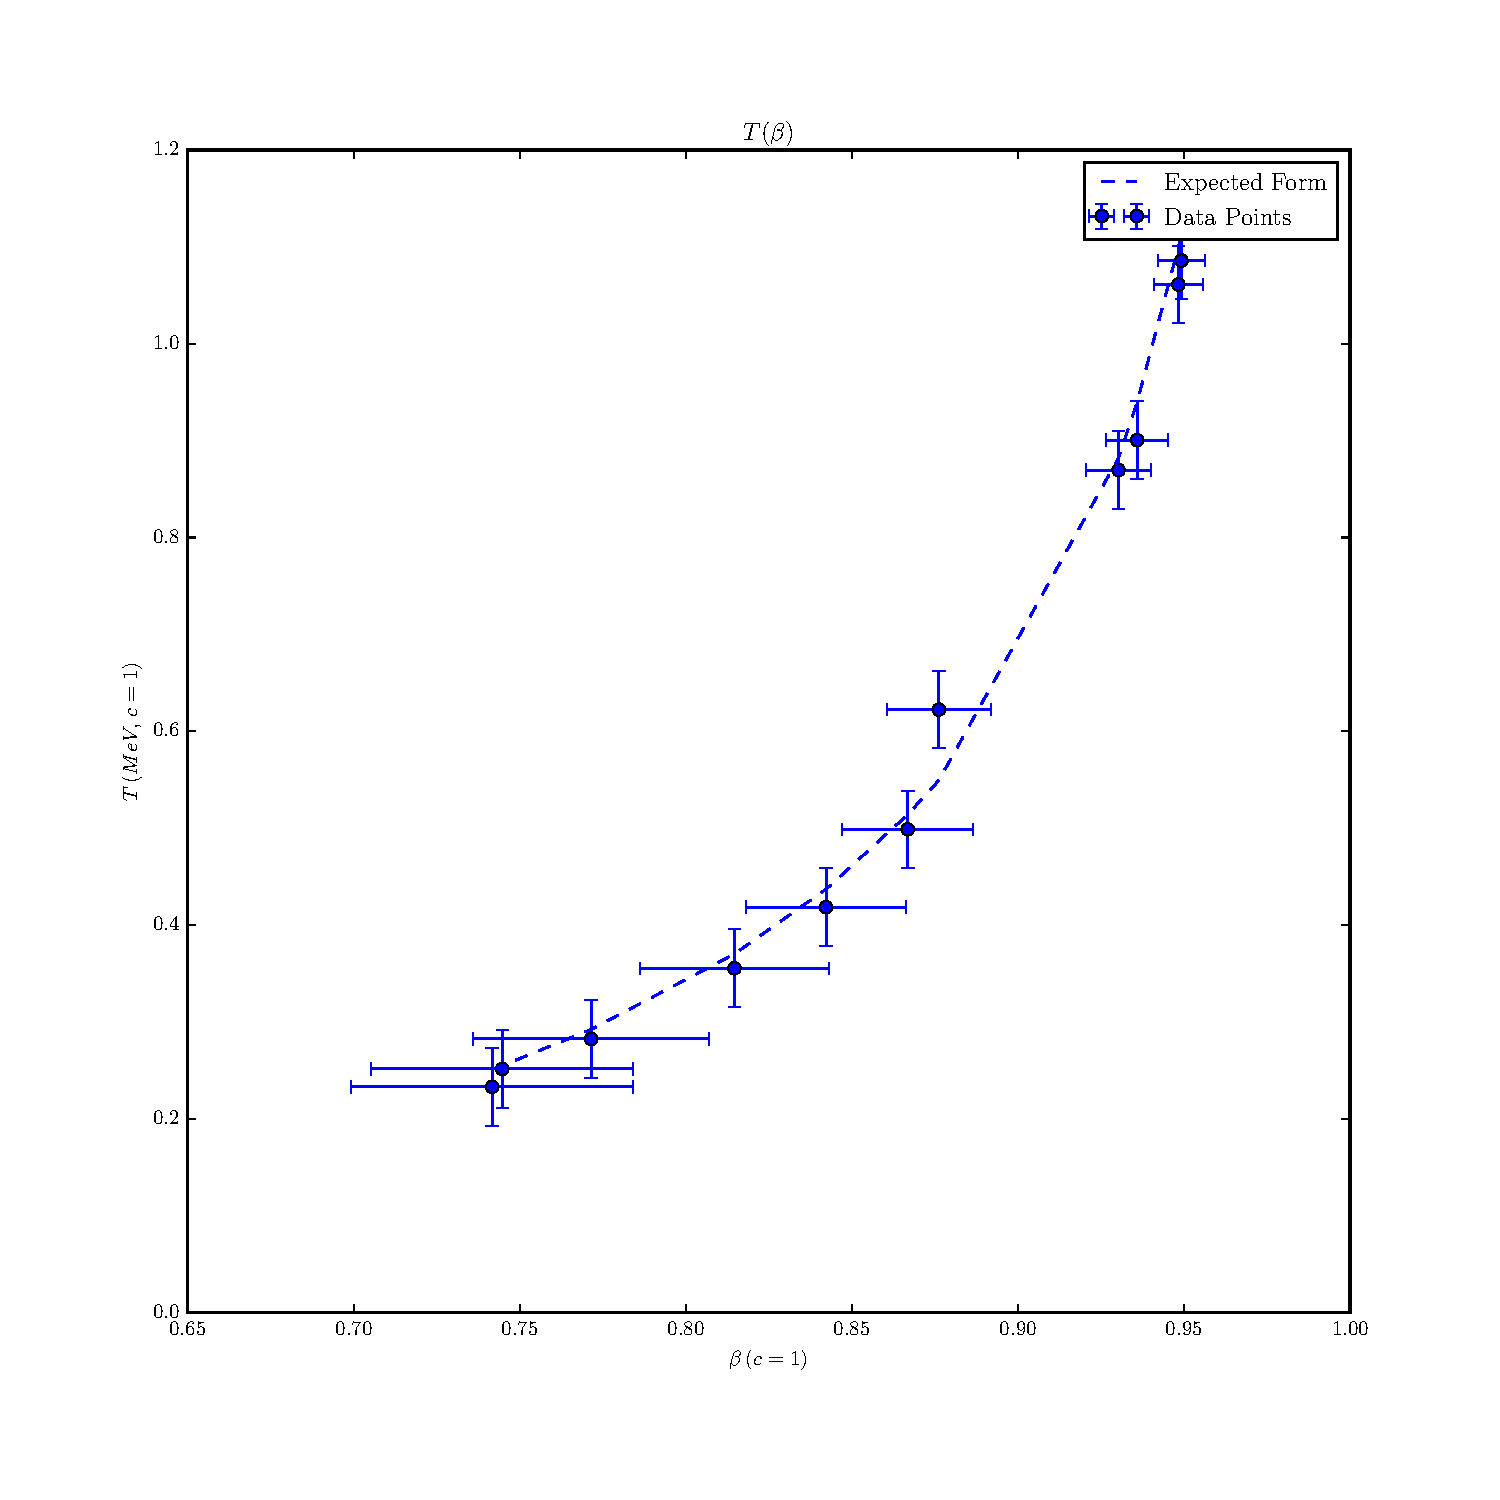
\includegraphics[width=\linewidth]{../plots/energyvsspeed.pdf}
        \caption{This is again to show similarities between the relativistic expression for kinetic energy and the data taken from these electrons. \label{fig:energyvsspeed}}
      \end{figure}

      \begin{figure}[h]
        \centering
        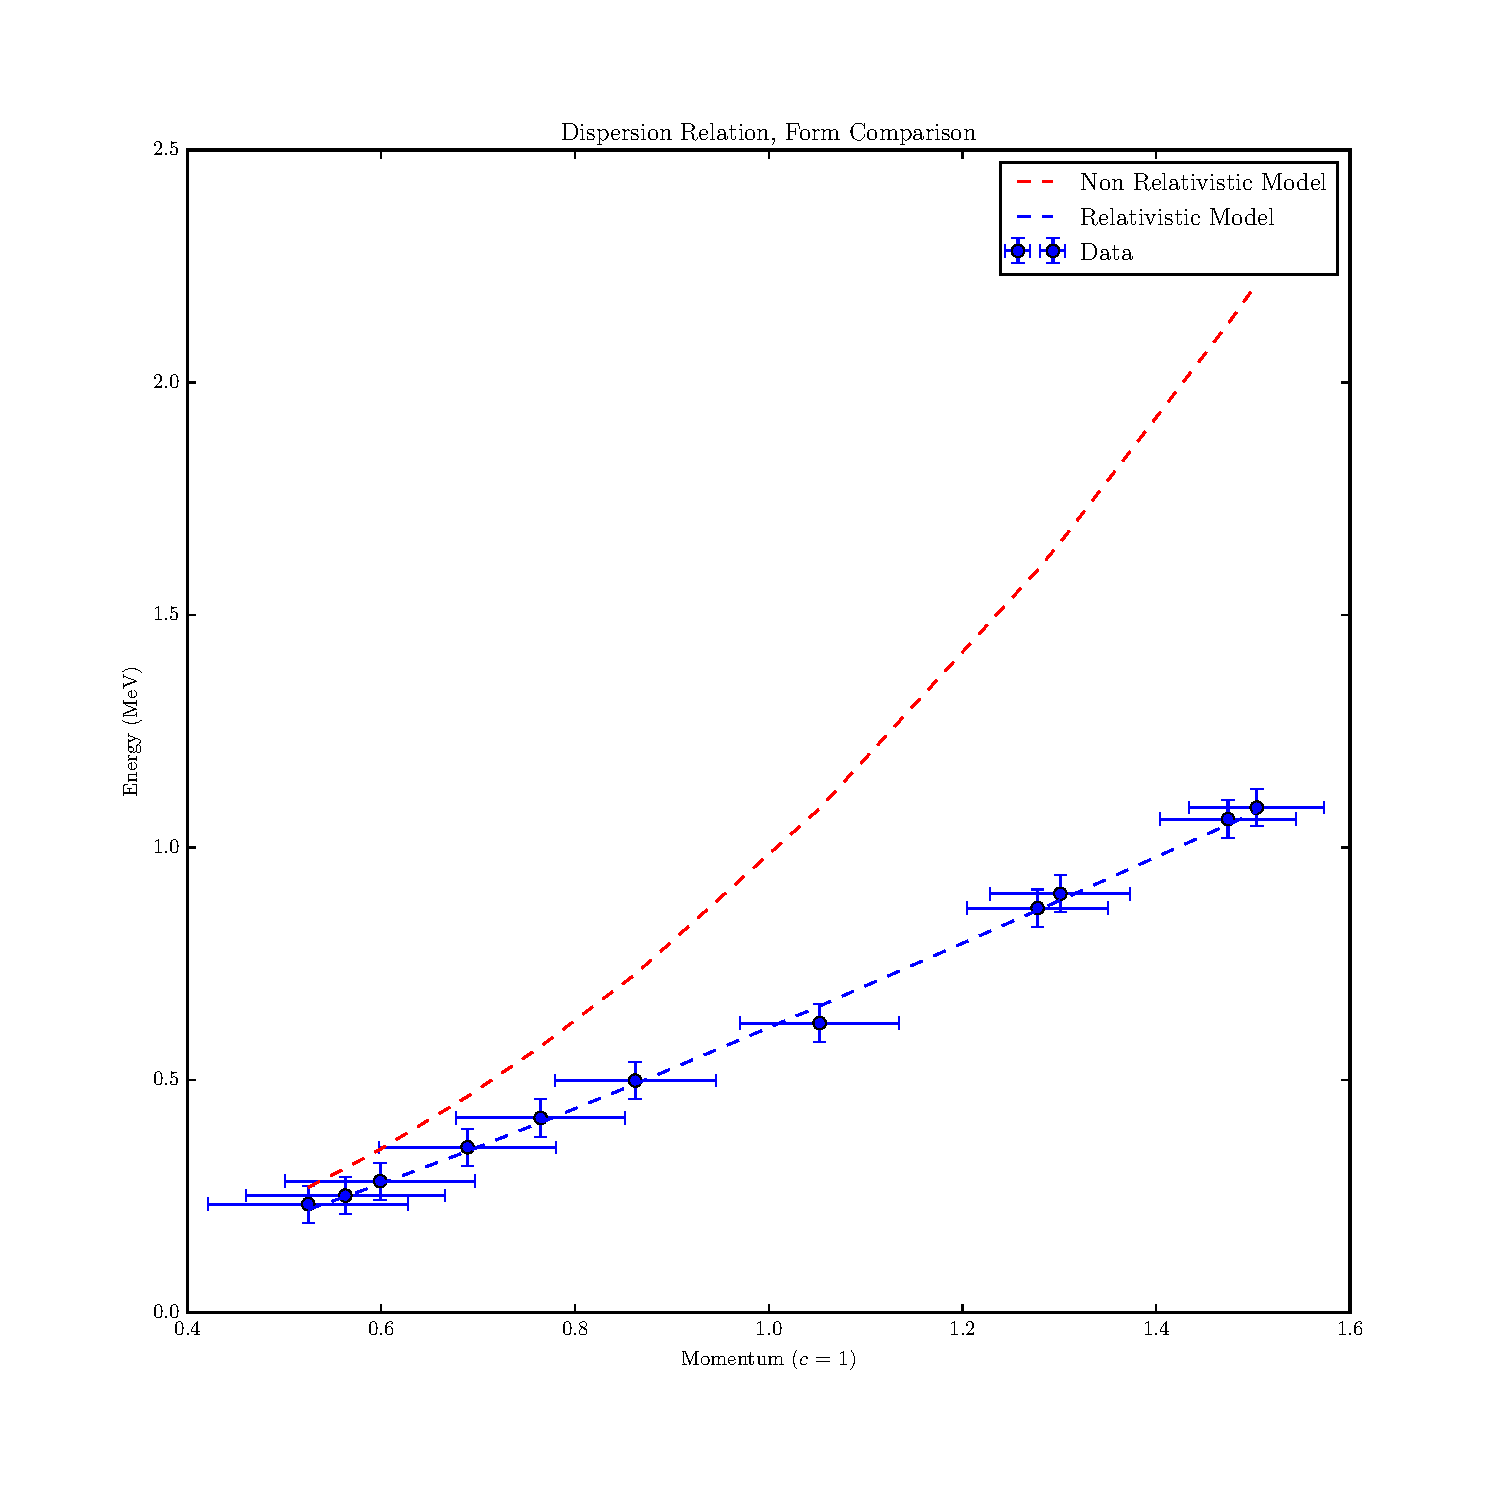
\includegraphics[width=\linewidth]{../plots/rel_dispersion.pdf}
        \caption{Moving at relativistic speeds flattens the band quite a bit as is evidenced here.  It also becomes obvious that the classical $p^2/2m$ relation does not hold at significant fractions of $c$. \label{fig:rel_dispersion}}
      \end{figure}
    \end{widetext}


\bibliography{bib}
\bibliographystyle{plain}

\end{document}
